\documentclass[11pt]{article}
\pdfoutput=1

\usepackage{./preamble}

\usepackage[T1]{fontenc}
\usepackage{newtxtext}
\usepackage{fullpage}
\usepackage{verbatim}
\usepackage[english]{babel}
\usepackage{tocloft}
\usepackage[x11names]{xcolor}

% Math.
\usepackage{amsmath,amsthm,amssymb,amscd,amsfonts,mathtools,mathrsfs,braket,bbm,enumerate,graphicx,bm,tcolorbox,physics}

% Remove period after theorem statement.
\newtheoremstyle{definition_no_period}
  {\parskip}    % ABOVESPACE
  {\parskip}    % BELOWSPACE
  {\normalfont} % BODYFONT
  {}            % INDENT (empty value is the same as 0pt)
  {\bfseries}   % HEADFONT
  {}            % HEADPUNCT
  {0.5em}       % HEADSPACE
  {}            % CUSTOM-HEAD-SPEC

\numberwithin{equation}{section}
%\usepackage{float}
\usepackage{tikz}
\usetikzlibrary{quantikz2}
\usepackage{algorithm,algpseudocode}
%\renewcommand{\thealgorithm}{}
\renewcommand{\algorithmicrequire}{\textbf{Input:}}
\renewcommand{\algorithmicensure}{\textbf{Output:}}
\allowdisplaybreaks

% Paragraph formatting.
\usepackage{parskip}
% For making parskip and theorem environments compatible.
\makeatletter
\def\thm@space@setup{%
  \thm@preskip=\parskip \thm@postskip=0pt
}
\makeatother

% Reference formatting.
\usepackage[pagebackref=true, colorlinks=true, linktoc=all, linkcolor=Blue3, citecolor=Turquoise3, urlcolor=Turquoise3]{hyperref}
\renewcommand*{\backrefalt}[4]{%
  \ifcase #1 \relax %
    \or \{#2\}%
    \else \{#2\}%
  \fi%
}
\renewcommand*{\backreftwosep}{, }
\renewcommand*{\backreflastsep}{, }
\usepackage[capitalise,nameinlink]{cleveref}

% For table of contents.
\makeatletter
%\@addtoreset{section}{part}
\makeatother
\newlength\mylen
\renewcommand\thepart{\Roman{part}}
\renewcommand\cftpartpresnum{Part~}
\settowidth\mylen{\bfseries\cftpartpresnum\cftpartaftersnum}
\addtolength\cftpartnumwidth{\mylen}
%\renewcommand{\cftpartleader}{\cftdotfill{\cftdotsep}}
\renewcommand{\cftsecleader}{\cftdotfill{\cftdotsep}}

% For authorship formatting.
\usepackage{authblk}
\renewcommand*{\Authsep}{\qquad}
\renewcommand*{\Authands}{\qquad}
\usepackage[para]{footmisc}
\newcommand*{\email}[1]{\href{mailto:#1}{\nolinkurl{#1}} }


% Theorem formatting. Have to use hooks after cleveref update.
\theoremstyle{definition_no_period}
% definitions
\newtheorem{definition}{Definition}[section]
% results
\newtheorem{result}{Result}[section]
\newtheorem{theorem}[result]{Theorem}\AddToHook{env/theorem/begin}{\crefalias{result}{theorem}}
\newtheorem{proposition}[result]{Proposition}\AddToHook{env/proposition/begin}{\crefalias{result}{proposition}}
\newtheorem{lemma}[result]{Lemma}\AddToHook{env/lemma/begin}{\crefalias{result}{lemma}}
\newtheorem{corollary}[result]{Corollary}\AddToHook{env/corollary/begin}{\crefalias{result}{corollary}}
\newtheorem{fact}[result]{Fact}\AddToHook{env/fact/begin}{\crefalias{result}{fact}}
\newtheorem{claim}[result]{Claim}\AddToHook{env/claim/begin}{\crefalias{result}{claim}}
% remarks
\newtheorem{remark}{Remark}[section]
\newtheorem{example}[remark]{Example}\AddToHook{env/example/begin}{\crefalias{remark}{example}}
\theoremstyle{plain}
% problems
\newtheorem{problem}{Problem}[section]
\newtheorem{conjecture}[problem]{Conjecture}\AddToHook{env/conjecture/begin}{\crefalias{problem}{conjecture}}
\newtheorem{task}[problem]{Task}\AddToHook{env/task/begin}{\crefalias{problem}{task}}


\DeclareMathOperator*{\argmin}{argmin}
\DeclareMathOperator*{\argmax}{argmax}
\DeclareMathOperator{\poly}{poly}
\renewcommand{\tr}{\operatorname{Tr}}
\DeclareMathOperator{\re}{Re}
\DeclareMathOperator{\im}{Im}
\DeclareMathOperator{\img}{im}
\DeclareMathOperator{\supp}{supp}
\DeclareMathOperator{\dist}{dist}
\renewcommand{\P}{\operatorname{\mathbf{P}}}
\DeclareMathOperator{\pr}{Pr}



\newcommand{\kk}[1]{{\color{red} KK: #1}}


%%%%%%%%%%%%%%%%%%%%%%%%%%%%%%%%%%%%%%%%%%%%%%%%%%%%%%%%%%%%%%%%%%%%%%%%%%%%%%%%%
%\title{CS4268 Scribe Notes}
% \author[1,2]{Everyone}
% \affil[1]{Centre for Quantum Technologies, NUS}
% \affil[2]{Department of Computer Science, NUS}

\begin{document}
%\maketitle
\begin{titlepage}
\vspace*{\fill}
\begin{center}

{\Large \textbf{CS4268 Lecture Notes}}\\
\vspace{1cm}
AY2025/26 Semester 2\\
\vspace{1cm}
CQT and SOC, NUS
\end{center}
\vspace*{\fill}
\end{titlepage}

\tableofcontents
\newpage

%change 'scribe templates' to 'final notes' later on for all such entries
% %%%% CUSTOM PREAMBLE
% \usepackage{./preamble}

% %% ADD MISC DEFINITIONS HERE %%%%%%%%%%%%%%%%%%%%%%%%%%%%%%%%%%%

% %%%%%%%%%%%%%%%%%%%%%%%%%%%%%%%%%%%%%%%%%%%%%%%%%%%%%
% %\addtolength{\topmargin}{-1cm}
% %\addtolength{\textheight}{2cm}

% \begin{document}


%\maketitle

\newpage
 %%*****************************************************
\noindent
\textbf{CS4268 AY2025-26 Sem 2}
\\
\noindent
Lecturer: Divesh Aggarwal
\hfill
Lecture 1                      %%% FILL IN LECTURE NUMBER HERE
\hfill
Date: January 15, 2026          %%% FILL IN LECTURE DATE HERE


\noindent
\rule{\textwidth}{1pt}

\medskip

%%%%%%%%%%%%%%%%%%%%%%%%%%%%%%%%%%%%%%%%%%%%%%%%%%%%%%%%%%%%%%%%
%% BODY OF SCRIBE NOTES GOES HERE
%%%%%%%%%%%%%%%%%%%%%%%%%%%%%%%%%%%%%%%%%%%%%%%%%%%%%%%%%%%%%%%%

\section{Introduction}
Quantum computing lies at the intersection of computer science, mathematics, and physics. It utilizes quantum mechanical laws to solve some complex problems (potentially) faster than classical computers. In this course, we shall take the laws of quantum mechanics for granted as our axiomatic "ground truth" and shall focus entirely on their \textbf{computational consequences} \cite{NC10}.

\subsection{Common Computational Tasks}
Let's first look at some common computational tasks and their complexities on classical computers.

\paragraph{Multiplication}
The classical primary-school (grid) algorithm for multiplying two \(n\)-digit numbers performs all digit-wise products explicitly and therefore requires a total of \(O(n^{2})\) single-digit operations. This was improved by Karatsuba, who introduced a divide-and-conquer strategy that reduces the multiplication of two \(n\)-digit numbers to three multiplications of size \(n/2\) (with some lower-order additions). Hence we get the recursion
\[
        T(n) = 3T(n/2) + O(n).
\]
yielding an overall time complexity of \(O\!\left(n^{\log_{2} 3}\right) \approx O\!\left(n^{1.58}\right)\).

The fastest known classical algorithms for multiplication go even further by utilizing the Fast Fourier Transform (FFT). For example, the Schönhage--Strassen algorithm for integer multiplication achieves a runtime of \(O(n \log n \log \log n)\) using FFT-based convolutions.

\paragraph{Factorization}
The simplest (and most direct) algorithm for factorizing an integer is \emph{trial division}. It finds a nontrivial divisor by checking integers $d = 2, 3, 4, \ldots$ and stopping when $d^2 > N$. This bound works because if $N = ab$ with $a \le b$, then $a \le \sqrt{N}$, and if no divisor exists up to $\sqrt{N}$, then $N$ is prime.

In the worst case, this algorithm requires $O(\sqrt{N})$ divisions, or a net $O(\sqrt{N})$ number of arithmetic operations. If the input size is $n$ (where $n = \log_2 N$= number of bits), then
\[
\sqrt{N} = 2^{\frac{1}{2} \log_2 N} = 2^{n/2}.
\]
Thus, trial division has a runtime of $O(2^{n/2})$ and is exponential in the bit length of the input. Hence, this algorithm quickly becomes infeasible for practical use as the input size increases.

The most efficient known classical algorithm for factorization is the \emph{General Number Field Sieve} (GNFS). Its runtime is
\[
\exp\!\left( \left( \frac{64}{9} \right)^{1/3} (\log N)^{1/3} (\log \log N)^{2/3} \right),
\]
which is sub-exponential in $N$ but still super-polynomial in the input size, making it once again infeasible for practical use when $N$ is large.

\medskip
\noindent
\fbox{%
    \parbox{\textwidth}{%
        \textbf{RSA}\\
        The apparent hardness of factorizing large numbers, especially semiprimes (numbers that are a product of two large primes) is what is utilized by the RSA public key cryptosystems, widely deployed in practice. It exploits the fact that given a huge semiprime $N$ (where $N = pq$ and both $p$ and $q$ are large prime numbers satisfying some sanity checks), it is hard to factorize the number and find $p$ and $q$.
    }%
}
\medskip

\paragraph{Unstructured Database Search}
In the unstructured database search problem, the idea is that given a bit string $a_1a_2...a_n$, suppose it is promised that exactly one position contains 1 and rest all are 0s. The goal is to find the unique position \( i \) for which \( a_i = 1 \).

The classical deterministic approach to this problem is the brute force search algorithm. It checks all \( n \) possibilities in the input and finds the correct \( i \) for which \( a_i = 1 \) in an overall runtime of \( O(n) \). In the deterministic setting, it is easy to see that $\Omega(n)$ is a lower bound as well. Even if we allow classical randomized computation, it can be shown that we still have a complexity of $\Theta(n)$ for this problem.

\subsection{Probabilistic Computing}

Probabilistic computing consists of randomized algorithms that, in addition to the input, also have access to a source of randomness such as independent and unbiased coin tosses. Due to the source of randomness the algorithm may lead to different execution paths for the same inputs.

Randomized algorithms can usually be divided into two types: Monte Carlo algorithms and Las Vegas algorithms. Monte Carlo algorithms are those that always terminate within a prescribed polynomial time bound but may return an incorrect answer with some bounded probability. Las Vegas algorithms on the other hand always produce a correct output, but their running time is a random variable whose expected value is usually polynomial.

\paragraph{Primality Testing}
One of the primary problems where randomized algorithms prove to be useful is primality testing. The goal here is to identify whether the input number is prime or composite. As discussed earlier, deterministic trial division takes \( O(2^{n/2}) \) time for this.

The Miller-Rabin test, on the other hand, uses Monte Carlo primality testing to achieve a complexity of \( O(n^{2} \log n \log \log n) \), which is polynomial in the input size. Solovay--Strassen \cite{SolovayStrassen77} is another randomized algorithm that achieves this task in a runtime of \( O(k \log^{3} n) \), where \( k \) is the number of tested bases. It was only very recently (2002) that a deterministic algorithm for primality testing was found. The AKS algorithm \cite{AKS04} provably runs in an overall time of \( O(\log^{12} N) \). Subsequent improvements under specific assumptions reduces this to \( O(\log^{6} N) \) \cite{LenstraPomerance19}.

\medskip
\noindent
\fbox{%
    \parbox{\textwidth}{%
        \textbf{BPP = P}\\
        A very strongly held belief in the theoretical computation community is that $\mathbf{BPP} = \mathbf{P}$. 
This means that any problem that can be solved in polynomial time with bounded error probability (using randomness) can also be solved in polynomial time deterministically. If true, this would formalize the idea that random bits are merely a convenience for designing faster algorithms, and not a fundamentally stronger computational resource. This remains officially unproven, however.
    }%
}
\medskip

\subsection{Role of Quantum Computing}
As discussed earlier, quantum computing utilizes the principles of quantum mechanics to implement algorithms that can solve specific complex problems better than classical computers. Two examples for this are as follows which we shall see in details in this course:
\begin{enumerate}
    \item \textbf{Shor's Algorithm (1994):} Peter Shor discovered a quantum algorithm that can factor integers in \textbf{polynomial time}. This gives an exponential speedup than the best known classical counterpart.
    \begin{itemize}
        \item \textit{Implication:} If we can build a large-scale quantum computer, there is an "easy" way of factorizing the product of 2 large prime numbers effectively breaking the public-key RSA cryptography. 
    \end{itemize}
    
    \item \textbf{Grover's Algorithm (1996):} Lov Grover discovered a way to solve the unstructured database search problem on a quantum computer in time $O(\sqrt{n})$, which can be proved to be the lower bound as well making its quantum complexity to be $\Theta(\sqrt{n})$, which is a quadratic speedup than its classical counterpart.
    \begin{itemize}
        \item \textit{Implication:} Its application also extends to a number of other problems, such as the Boolean Satisfiability (SAT) problem. The goal of this problem is to determine whether a Boolean formula with \( n \) variables has an assignment that makes it evaluate to true. A deterministic exhaustive search would require testing all \( 2^{n} \) possible assignments, whereas Grover’s algorithm can find a satisfying assignment in approximately \( 2^{n/2} \) steps. Thus, although the runtime remains exponential, the algorithm achieves a quadratic reduction. Consequently, Grover’s algorithm does not reduce NP-complete problems to polynomial time, but it effectively halves the exponent in their time complexity.
    \end{itemize}
\end{enumerate}




\section{The Fundamental Axioms of Quantum Mechanics}

In the previous section, we saw that probabilistic computing is "Classical Computing + Randomness."
Quantum computing introduces something richer: interference via superposition and entanglement. A high-level summary is:
\[
    \text{Quantum Computing} = \text{Classical Computing} + \text{Interference (Rotation)}.
\]
While probabilistic algorithms introduce randomness via coin tosses, quantum computing uses this extra structure to manipulate information in ways classical computers cannot. This is the source of quantum speedups:
\begin{itemize}
    \item \textbf{Polynomial Speedups:} For problems like unstructured search (Grover's Algorithm).
    \item \textbf{Exponential Speedups:} For problems like factoring (Shor's Algorithm). \cite{NC10}
\end{itemize}

Since quantum states behave like \textbf{vectors} that can be rotated, to understand these algorithms, we must rely heavily on \textbf{Linear Algebra}.

\subsection{From Bits to Qubits}

A classical bit has a state $x \in \{0, 1\}$.
A quantum bit, or \textbf{qubit}, also has two basis states, which we label using the standard "ket" notation:
\[
    \ket{0} \quad \text{and} \quad \ket{1}.
\]
For now, treat $\ket{0}$ and $\ket{1}$ as abstract labels. However, intuition comes from physics, where objects can be in more than one state at the same time:
\begin{itemize}
    \item An \textbf{electron} may have two energy levels, labeled $0$ (ground) and $1$ (excited).
    \item A \textbf{photon} may have polarization that is Horizontal or Vertical.
\end{itemize}
If we label Horizontal as $\ket{0}$ and Vertical as $\ket{1}$, then before measurement, the photon may be in a superposition of both. After measurement, we observe only one outcome.

\subsection{Law 1: Superposition}

The first fundamental difference is that a qubit can be in a state that is a linear combination of the basis states.

\begin{definition}[Quantum Mechanics Law 1: Superposition] If a quantum particle can be in one of the 2 basis states $\ket{0}$ and $\ket{1}$, then it can also be in a superposition state:
\[
    \ket{\psi} = \alpha\ket{0} + \beta\ket{1},
\]
where $\alpha, \beta \in \mathbb{C}$ are complex numbers called \textbf{amplitudes}.
These amplitudes must satisfy the \textbf{normalization condition}:
\[
    |\alpha|^2 + |\beta|^2 = 1.
\]
\end{definition}

\paragraph{Geometric Intuition (The Unit Circle)}
If we restrict ourselves to \textbf{real} amplitudes ($\alpha, \beta \in \mathbb{R}$), the condition $\alpha^2 + \beta^2 = 1$ describes a circle of radius 1.
Thus, we can visualize the state of a qubit as a point on the unit circle in $\mathbb{R}^2$.

\begin{example}
Consider the state $\ket{\psi} = 0.8\ket{0} - 0.6\ket{1}$.
Check normalization:
\[
    |0.8|^2 + |-0.6|^2 = 0.64 + 0.36 = 1.
\]
Geometrically, this corresponds to the point $(0.8, -0.6)$ on the unit circle.
\end{example}

\begin{remark}[Complex Amplitudes]
In the general case, $\alpha$ and $\beta$ are complex numbers ($a + ib$). The magnitude is defined as $|\alpha| = \sqrt{a^2 + b^2}$. For example, if $\ket{\psi} = \frac{1}{\sqrt{2}}\ket{0} + \frac{i}{\sqrt{2}}\ket{1}$, then $|\frac{i}{\sqrt{2}}|^2 = \frac{1}{2}$.
\end{remark}

\subsection{Law 2: Measurement}
We cannot "see" the amplitudes $\alpha$ and $\beta$ directly. We can only extract information via measurement.

\begin{definition}[Quantum Mechanics Law 2: Measurement]
Given a state $\ket{\psi} = \alpha\ket{0} + \beta\ket{1}$, if we measure it in the standard basis:
\begin{enumerate}
    \item We observe outcome $\ket{0}$ with probability $P(0) = |\alpha|^2$.
    \item We observe outcome $\ket{1}$ with probability $P(1) = |\beta|^2$.
\end{enumerate}
Crucially, after the measurement, the state \textbf{collapses} to the observed outcome.
\end{definition} 
\begin{example}
    Suppose we have the state $\ket{\psi} = 0.8\ket{0} + 0.6\ket{1}$.
    \begin{itemize}
        \item \textbf{Probability:} We see $\ket{0}$ with probability $0.64$, and $\ket{1}$ with probability $0.36$.
        \item \textbf{Collapse:} If we see $\ket{0}$, the state \textit{becomes} $\ket{0}$. A second measurement will yield $\ket{0}$ with 100\% probability.
    \end{itemize}
\end{example}

This is the key distinction from simply "revealing" a hidden coin toss. In the quantum world, the measurement forces the system to choose a reality.

\subsection{The Mathematical Formalism: Qubits as Vectors}

So far, we have used $\ket{0}$ and $\ket{1}$ as abstract labels. Mathematically, a quantum state is a vector in a complex vector space $\mathbb{C}^d$.
For a single qubit, the dimension is $d=2$. We identify the basis states with the standard basis vectors:
\[
    \ket{0} = e_0 = \begin{bmatrix} 1 \\ 0 \end{bmatrix}, \qquad
    \ket{1} = e_1 = \begin{bmatrix} 0 \\ 1 \end{bmatrix}.
\]
Consequently, a general superposition $\ket{\psi} = \alpha\ket{0} + \beta\ket{1}$ is simply a column vector:
\[
    \ket{\psi} = \alpha \begin{bmatrix} 1 \\ 0 \end{bmatrix} + \beta \begin{bmatrix} 0 \\ 1 \end{bmatrix} = \begin{bmatrix} \alpha \\ \beta \end{bmatrix} \in \mathbb{C}^2.
\]

\subsection{Beyond Two-Basis States: Qudits and General Laws}

There is nothing special about having exactly two states.
\begin{itemize}
    \item A \textbf{qutrit} ($d=3$) has basis states $\ket{0}, \ket{1}, \ket{2}$.
    \item A general \textbf{qudit} ($d$) has basis states $\ket{0}, \ket{1}, \dots, \ket{d-1}$.
\end{itemize}

In this general setting, the state is a vector in $\mathbb{C}^d$:
\[
    \ket{\psi} = \alpha_0\ket{0} + \dots + \alpha_{d-1}\ket{d-1} \iff \begin{bmatrix} \alpha_0 \\ \vdots \\ \alpha_{d-1} \end{bmatrix} \in \mathbb{C}^d.
\]
Each basis state $\ket{i}$ is the standard basis vector $e_i$ (a column with a $1$ in the $i$-th position and $0$ elsewhere).

We can now restate our two fundamental laws in their full generality.

\begin{definition}[Law 1 in dimension $d$: State]
A general $d$-dimensional state is a superposition:
\[
    \ket{\psi} = \sum_{i=0}^{d-1} \alpha_i \ket{i}, \quad \text{subject to} \quad \sum_{i=0}^{d-1} |\alpha_i|^2 = 1.
\]
\end{definition}

\begin{definition}[Law 2 in dimension $d$: Measurement]
Measuring $\ket{\psi} = \sum \alpha_i \ket{i}$ outputs outcome $i$ with probability $|\alpha_i|^2$.
Immediately after measurement, the state collapses to $\ket{i}$.
\end{definition}

\paragraph{An example: a 4-dimensional system \texorpdfstring{($d=4$)}{(d=4)}}

A common example is $d=4$. We can view this as a single system with 4 levels ($\ket{0}, \ket{1}, \ket{2}, \ket{3}$), or deeply importantly, as a system of \textbf{two qubits}.
If we have two qubits, the combined system has $2 \times 2 = 4$ basis states:
\[
    \ket{00}, \ket{01}, \ket{10}, \ket{11}.
\]
Here, $\ket{01}$ means "First qubit is 0, Second qubit is 1." This scaling ($2^n$ dimension for $n$ qubits) is the source of quantum computing's massive state space.



% \bibliographystyle{alpha}
% \bibliography{main}

% \end{document} 
\newpage

% %%%% CUSTOM PREAMBLE
% \usepackage{./preamble}

% %% ADD MISC DEFINITIONS HERE %%%%%%%%%%%%%%%%%%%%%%%%%%%%%%%%%%%

% %%%%%%%%%%%%%%%%%%%%%%%%%%%%%%%%%%%%%%%%%%%%%%%%%%%%%
% %\addtolength{\topmargin}{-1cm}
% %\addtolength{\textheight}{2cm}

% \begin{document}


%\maketitle
\newpage
\noindent
\textbf{CS4268 AY2025-26 Sem 2}
\\
\noindent
Lecturer: Divesh Aggarwal
\hfill
Lecture 2                      %%% FILL IN LECTURE NUMBER HERE
\hfill
Date: January 22, 2026          %%% FILL IN LECTURE DATE HERE


\noindent
\rule{\textwidth}{1pt}

\medskip

\section{Hilbert Space and Quantum States}
The language of quantum mechanics is linear algebra. We shall assume some familiarity with it, but introduce a very useful bookkeeping tool -- Dirac's bra-ket notation.

\subsection{Hilbert Space}

Recall the notion of a Hilbert Space.
\begin{definition}[Hilbert Space]
A \textbf{Hilbert Space} $\mathcal{H}$ over $\mathbb{C}$ is a complete vector space over the complex numbers equipped with an inner product $\langle \cdot, \cdot \rangle : \mathcal{H} \times \mathcal{H} \to \mathbb{C}$ that satisfies:
\begin{itemize}
\item Conjugate symmetry: $\langle u, v \rangle = \overline{\langle v, u \rangle}$
\item Linearity in the second argument: $\langle u, \alpha v + \beta w \rangle = \alpha \langle u, v \rangle + \beta \langle u, w \rangle$ for $\alpha, \beta \in \mathbb{C}$
\item Positive definiteness: $\langle v, v \rangle \geq 0$ with equality if and only if $v = 0$
\end{itemize}
\end{definition}

\subsection{Dirac's Bra-Ket Notation}

Dirac's bra-ket notation:
\begin{definition}[Bra-ket Notation]
A \textbf{ket} $\ket{v}$ denotes a column vector in the Hilbert space $\mathcal{H}$.
\begin{itemize}
\item Basis vectors are denoted $\ket{0}, \ket{1}, \ldots, \ket{n-1}$ for an $n$-dimensional space.
\item A general vector can be written as a linear combination: $\ket{\psi} = \sum_{i} \alpha_i \ket{i}$ where $\alpha_i \in \mathbb{C}$.
\item A \textbf{bra} $\bra{v}$ denotes the conjugate transpose of $\ket{v}$, i.e., $\bra{v} = (\ket{v})^\dagger$, which is a row vector.
\item The inner product of two vectors $\ket{u}$ and $\ket{v}$ is written as $\langle u|v \rangle$.
\item Orthonormality of basis vectors: $\langle i|j \rangle = \delta_{ij}$.
\end{itemize}
\end{definition}

\begin{remark}[Conjugate Transpose as Bra]
Given a ket
\[
\ket{v} = \begin{pmatrix} v_1 \\ \vdots \\ v_d \end{pmatrix} \in \C^d,
\]
its bra is the conjugate transpose
\[
\bra{v} = (\ket{v})^\dagger = \big(v_1^*, \ldots, v_d^*\big).
\]
The inner product is therefore
\[
\langle u|v \rangle = u^\dagger v,
\]
which suppresses explicit matrix multiplication and should be read as ``bra-$u$ ket-$v$''.
\end{remark}

\begin{example}[Notations for Bases]
Dirac's notation unifies familiar notions of basis vectors:

\begin{itemize}
    \item \textbf{High school basis (in $\R^3$):}
    \[
        \hat{i} = \begin{pmatrix} 1 \\ 0 \\ 0 \end{pmatrix},\quad
        \hat{j} = \begin{pmatrix} 0 \\ 1 \\ 0 \end{pmatrix},\quad
        \hat{k} = \begin{pmatrix} 0 \\ 0 \\ 1 \end{pmatrix}
    \]

    \item \textbf{Linear algebra basis in $\R^d$ (standard basis):}
    \[
        e_1 = \begin{pmatrix} 1 \\ 0 \\ \vdots \\ 0 \end{pmatrix},\quad
        e_2 = \begin{pmatrix} 0 \\ 1 \\ \vdots \\ 0 \end{pmatrix},\quad
        \ldots,\quad
        e_d = \begin{pmatrix} 0 \\ 0 \\ \vdots \\ 1 \end{pmatrix}
    \]

    \item \textbf{Quantum computational basis in $\C^d$:}
    \[
        \ket{0} = \begin{pmatrix} 1 \\ 0 \\ 0 \\ \vdots \\ 0 \end{pmatrix},\quad
        \ket{1} = \begin{pmatrix} 0 \\ 1 \\ 0 \\ \vdots \\ 0 \end{pmatrix},\quad
        \ket{2} = \begin{pmatrix} 0 \\ 0 \\ 1 \\ \vdots \\ 0 \end{pmatrix},\quad
        \ldots,\quad
        \ket{d-1} = \begin{pmatrix} 0 \\ 0 \\ \vdots \\ 1 \end{pmatrix}
    \]
\end{itemize}

In an $n$-dimensional quantum system (e.g., qubit: $n=2$, qutrit: $n=3$, qudit: $n=d$), these vectors form the \emph{computational basis} $\{\ket{0},\ket{1},\ldots,\ket{n-1}\}$ and satisfy
\[
\langle i|j \rangle = \delta_{ij}.
\]
\end{example}

\begin{example}[Complex Vector Example]
Consider the vector
\[
\ket{v} = \frac{1}{13}
\begin{pmatrix}
3 + 4i \\
12i
\end{pmatrix}.
\]
Then the corresponding bra is
\[
\bra{v}
= \frac{1}{13}\big(3 - 4i,\; -12i\big),
\]
obtained by taking the conjugate transpose of the ket.
\end{example}

\subsection{Quantum States}

From now on everything is denoted in bra-ket notation.

In quantum mechanics a system is mathematically modelled by a suitable (to be determined from theory and experiment) Hilbert space. The quantum state representing the system is simply an element of this Hilbert space.
% \begin{definition}
%     Add quantum state as element of Hilbert space, as superposition of basis vectors, column vector representation. Add physical interpretation of the components $\alpha_i$ of the column vector.
% \end{definition}
\begin{definition}[Quantum State]
A \textbf{quantum state} $\ket{\psi}$ is an element of a Hilbert space $\mathcal{H}$ with unit norm, i.e., $\langle \psi|\psi \rangle = 1$.

For a quantum system with orthonormal basis $\{\ket{0}, \ket{1}, \ldots, \ket{n-1}\}$, any quantum state can be written as a superposition:
$$\ket{\psi} = \sum_{i=0}^{n-1} \alpha_i \ket{i} = \alpha_0 \ket{0} + \alpha_1 \ket{1} + \cdots + \alpha_{n-1} \ket{n-1}$$
where $\alpha_i \in \mathbb{C}$ are complex amplitudes satisfying the normalization condition $\sum_{i=0}^{n-1} |\alpha_i|^2 = 1$.

In column vector representation:
$$\ket{\psi} = \begin{pmatrix} \alpha_0 \\ \alpha_1 \\ \vdots \\ \alpha_{n-1} \end{pmatrix}.$$

\textbf{Physical Interpretation:} When we measure the quantum state $\ket{\psi}$ in the computational basis, the probability of observing outcome $i$ is $|\alpha_i|^2$. This is \textbf{Born's rule}.
\end{definition}

\begin{example}[Quantum States as Superpositions]
For a single qubit (2-dimensional quantum system):
\begin{itemize}
\item Computational basis states: $\ket{0} = \begin{pmatrix} 1 \\ 0 \end{pmatrix}$ and $\ket{1} = \begin{pmatrix} 0 \\ 1 \end{pmatrix}$

\item Superposition state: $\ket{+} = \frac{1}{\sqrt{2}}(\ket{0} + \ket{1}) = \frac{1}{\sqrt{2}}\begin{pmatrix} 1 \\ 1 \end{pmatrix}$

\item Another superposition: $\ket{-} = \frac{1}{\sqrt{2}}(\ket{0} - \ket{1}) = \frac{1}{\sqrt{2}}\begin{pmatrix} 1 \\ -1 \end{pmatrix}$

\item General qubit state: $\ket{\psi} = \alpha\ket{0} + \beta\ket{1}$ where $|\alpha|^2 + |\beta|^2 = 1$
\end{itemize}
The states $\ket{+}$ and $\ket{-}$ form the Hadamard basis (also called the $X$-basis or plus-minus basis).
\end{example}

Of course, we know the basis of a (nontrivial) Hilbert space is not unique. We could choose to represent states w.r.t. different bases, so the corresponding column vectors would have different physical interpretations.

\section{Measurements in different bases and the Elitzur-Vaidman Test}
\subsection{Measurements in Different Bases}
Up until now, we have only considered measurements with respect to the standard basis ($\{ \ket{0}, \ket{1} \}$ in the $2$ dimensional case). However, we are not restricted to just measuring in the standard basis and can use any valid set of orthonormal basis states as the measurement basis. Let us now consider the problem of making measurements with respect to different bases.
\begin{example}[Measurement with respect to Different Bases]
Consider a qubit in state $\ket{+} = \frac{1}{\sqrt{2}}(\ket{0} + \ket{1})$.

\textbf{Measurement w.r.t. computational basis $\{\ket{0}, \ket{1}\}$}:
\begin{itemize}
\item $\pr(\text{measure} \ket{0}) = |\frac{1}{\sqrt{2}}|^2 = \frac{1}{2}$,
\item $\pr(\text{measure} \ket{1}) = |\frac{1}{\sqrt{2}}|^2 = \frac{1}{2}$.
\end{itemize}

\textbf{Measurement w.r.t. Hadamard basis $\{\ket{+}, \ket{-}\}$}:

First, express $\ket{+}$ in the new basis. Since $\ket{0} = \frac{1}{\sqrt{2}}(\ket{+} + \ket{-})$ and $\ket{1} = \frac{1}{\sqrt{2}}(\ket{+} - \ket{-})$, we have:
$$\ket{+} = \frac{1}{\sqrt{2}}(\ket{0} + \ket{1}) = \frac{1}{\sqrt{2}}\left[\frac{1}{\sqrt{2}}(\ket{+} + \ket{-}) + \frac{1}{\sqrt{2}}(\ket{+} - \ket{-})\right] = 1 \cdot \ket{+} + 0 \cdot \ket{-}.$$

Thus
\begin{itemize}
\item $\pr(\text{measure} \ket{+}) = |1|^2 = 1$,
\item $\pr(\text{measure} \ket{-}) = |0|^2 = 0$.
\end{itemize}

\textbf{Key insight:} When we measure $\ket{+}$ in the Hadamard basis $\{\ket{+}, \ket{-}\}$, the coefficient of $\ket{+}$ is 1 and the coefficient of $\ket{-}$ is 0. This makes intuitive sense: if the system is already in state $\ket{+}$ and we measure in the $\{\ket{+}, \ket{-}\}$ basis, we are guaranteed to get the outcome $\ket{+}$. Thus, the same quantum state gives different measurement outcomes depending on the measurement basis.
\end{example}

\subsection{Elitzur-Vaidman Bomb-Tester}
Now let us consider the following thought experiment. Suppose we are given a box that is either a DUD or a bomb. We want to figure out which box we are given without triggering an explosion. The behaviour of the two possible boxes is shown below:
% Classical option and preliminary quantum option. Conclusions from these options.
\begin{center}
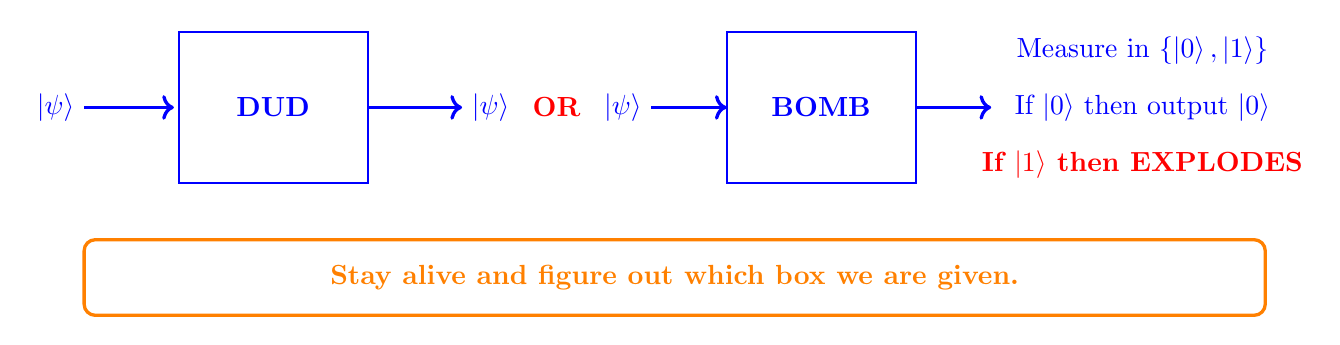
\begin{tikzpicture}[scale=1.2]
% Photon input
\draw[->, very thick, blue] (-1,0) -- (-0.05,0);
\node[left, blue] at (-1,0) {$\ket{\psi}$};

% First box - DUD
\draw[thick, blue] (0,-0.8) rectangle (2,0.8);
\node[blue] at (1,0) {\textbf{DUD}};

% Arrow from DUD
\draw[->, very thick, blue] (2,0) -- (3,0);
\node[right, blue] at (3,0) {$\ket{\psi}$};

% OR text with more space
\node[red, font=\bfseries] at (4.0,0) {OR};

% Arrow to bomb with spacing
\draw[->, very thick, blue] (5.0,0) -- (5.8,0);
\node[right, blue] at (4.4,0) {$\ket{\psi}$};

% Second box - BOMB
\draw[thick, blue] (5.8,-0.8) rectangle (7.8,0.8);
\node[blue] at (6.8,0) {\textbf{BOMB}};

% Arrow from BOMB to right
\draw[->, very thick, blue] (7.8,0) -- (8.6,0);

% Measure text (no arrow, just text aligned to the right)
\node[blue, align=left] at (10.2,0.6) {Measure in $\{\ket{0}, \ket{1}\}$};

% Outcomes
\node[blue, align=left] at (10.2, 0) {If $\ket{0}$ then output $\ket{0}$};
\node[red, align=left, font=\bfseries] at (10.2,-0.6) {If $\ket{1}$ then EXPLODES};

% Goal box at bottom
\draw[orange, very thick, rounded corners] (-1,-1.4) rectangle (11.5,-2.2);
\node[orange, font=\bfseries] at (5.25,-1.8) {Stay alive and figure out which box we are given.};
\end{tikzpicture}
\end{center}

Some preliminary options that comes to mind are sending $\ket{0}$ or $\ket{+}$ through the unknown box, and then measure the output from the box. Let us examine what happens in each of these cases.

\textbf{Classical Strategy:}

If we send $\ket{0}$, we are unable to identify if it is a dud or a bomb as the output is the same. If we send $\ket{1}$:
\begin{itemize}
\item No explosion $\Rightarrow$ it's a dud!
\item Bomb explodes $\Rightarrow$ it's a bomb! (but you dead)
\end{itemize}

\textit{Conclusion:} Classically impossible to distinguish dud/bomb without triggering an explosion.

\textbf{Preliminary Quantum Strategy:}

Send in $\ket{\psi} = \ket{+}$ and measure w.r.t. $\{\ket{+}, \ket{-}\}$.

\textit{Case 1: Dud bomb}

If it's a dud, we will always see $\ket{+}$ because 100\% of the amplitude is on $\ket{+}$.

\begin{center}
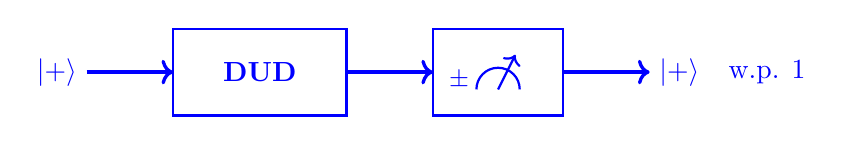
\begin{tikzpicture}[scale=1.1]
\draw[->, very thick, blue] (0,0) -- (1,0);
\node[left, blue] at (0,0) {$\ket{+}$};
\draw[thick, blue] (1,-0.5) rectangle (3,0.5);
\node[blue] at (2,0) {\textbf{DUD}};
\draw[->, very thick, blue] (3,0) -- (4,0);
\draw[thick, blue] (4,-0.5) rectangle (5.5,0.5);
% Measurement device with arc and arrow
\node[blue, font=\small] at (4.3,-0.1) {$\pm$};
\draw[blue, thick] (4.5,-0.2) arc[start angle=180, end angle=0, radius=0.25];
\draw[blue, thick, ->] (4.75,-0.2) -- (4.95,0.2);
\draw[->, very thick, blue] (5.5,0) -- (6.5,0);
\node[right, blue] at (6.5,0) {$\ket{+}$};
\node[right, blue] at (7.3,0) {w.p. 1};
\end{tikzpicture}
\end{center}

\textit{Case 2: Working bomb}

Three possible outcomes:
\begin{itemize}
\item Bomb measures $\ket{0}$ and explodes (with probability $\frac{1}{2}$).
\item Bomb measures $\ket{1}$ and does not explode:
\begin{itemize}
\item We observe $\ket{+}$ (with probability $\frac{1}{4}$): inconclusive (could be dud or working)
\item We observe $\ket{-}$ (with probability $\frac{1}{4}$): Working bomb identified!
\end{itemize}
\end{itemize}

\begin{center}
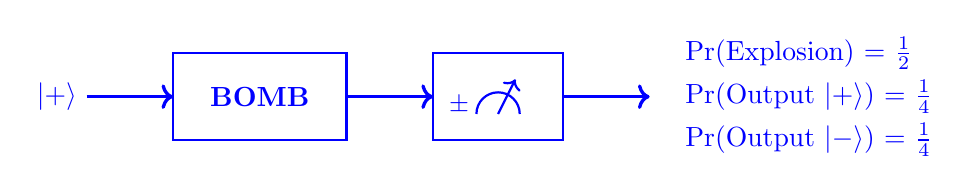
\begin{tikzpicture}[scale=1.1]
\draw[->, very thick, blue] (0,0) -- (1,0);
\node[left, blue] at (0,0) {$\ket{+}$};
\draw[thick, blue] (1,-0.5) rectangle (3,0.5);
\node[blue] at (2,0) {\textbf{BOMB}};
\draw[->, very thick, blue] (3,0) -- (4,0);
\draw[thick, blue] (4,-0.5) rectangle (5.5,0.5);
% Measurement device with arc and arrow
\node[blue, font=\small] at (4.3,-0.1) {$\pm$};
\draw[blue, thick] (4.5,-0.2) arc[start angle=180, end angle=0, radius=0.25];
\draw[blue, thick, ->] (4.75,-0.2) -- (4.95,0.2);
\draw[->, very thick, blue] (5.5,0) -- (6.5,0);
\node[blue, align=left, anchor=west] at (6.8,0.5) {$\pr$(Explosion) = $\frac{1}{2}$};
\node[blue, align=left, anchor=west] at (6.8,0) {$\pr$(Output $\ket{+}$) = $\frac{1}{4}$};
\node[blue, align=left, anchor=west] at (6.8,-0.5) {$\pr$(Output $\ket{-}$) = $\frac{1}{4}$};
\end{tikzpicture}
\end{center}

If we observe $\ket{-}$, we know it is a bomb because: with a dud, we get $\ket{+}$ all the time (with probability 1).

\textit{Conclusion:} $\frac{1}{4}$ success rate for identifying working bomb without explosion. 

\textbf{Can we improve upon this?} Yes.
First, but first let us make a brief detour into the notion of rotations (more generally, unitaries later on) on quantum states.

% \begin{definition}
%     Add material on rotations on a single qubit.
% \end{definition}
\subsection{Rotations and Reflections}

\paragraph{Rotations}

\begin{definition}[Rotations on a Single Qubit]
For any $\theta$, we can build a physical device that rotates a qubit by angle $\theta$. Consider a transformation that rotates the quantum state by a small angle $\theta$. Starting from $\ket{0}$, we apply a rotation:
$R(\theta): \ket{0} \mapsto \cos(\theta)\ket{0} + \sin(\theta)\ket{1}$

$$\ket{0} \to \begin{pmatrix} \cos\theta \\ \sin\theta \end{pmatrix}$$

$$\ket{1} \to \begin{pmatrix} \cos(\frac{\pi}{2} + \theta) \\ \sin(\frac{\pi}{2} + \theta) \end{pmatrix} = \begin{pmatrix} -\sin\theta \\ \cos\theta \end{pmatrix}$$

\begin{center}
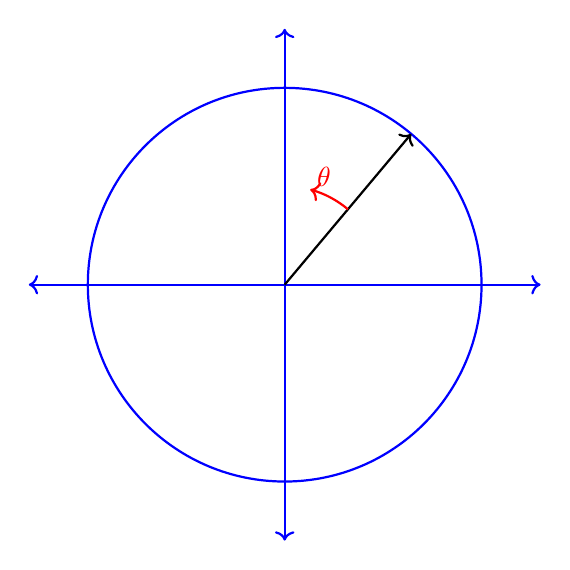
\begin{tikzpicture}[scale=2.5]
% Draw circle
\draw[thick, blue] (0,0) circle (1);
% Draw axes with arrows on both ends
\draw[thick, blue, <->] (-1.3,0) -- (1.3,0);
\draw[thick, blue, <->] (0,-1.3) -- (0,1.3);
% Draw vector at angle
\draw[thick, black, ->] (0,0) -- ({cos(50)},{sin(50)});
% Draw curved rotation arrow starting FROM the black arrow curving left, ending before vertical axis
\draw[thick, red, ->] ({0.5*cos(50)},{0.5*sin(50)}) arc (50:75:0.5);
\node[red] at (0.2,0.55) {$\theta$};
\end{tikzpicture}
\end{center}

For a general state $\alpha\ket{0} + \beta\ket{1}$, it gets transformed to:

\begin{align*}
\alpha\ket{0} + \beta\ket{1} &\to \alpha\begin{pmatrix} \cos\theta \\ \sin\theta \end{pmatrix} + \beta\begin{pmatrix} -\sin\theta \\ \cos\theta \end{pmatrix}\\
&\quad= \begin{pmatrix} \cos\theta & -\sin\theta \\ \sin\theta & \cos\theta \end{pmatrix} \begin{pmatrix} \alpha \\ \beta \end{pmatrix}
\
\end{align*}
where $\begin{pmatrix} 1 \\ 0 \end{pmatrix}$ goes to the vector $\begin{pmatrix} \cos\theta \\ \sin\theta \end{pmatrix}$ and $\begin{pmatrix} 0 \\ 1 \end{pmatrix}$ goes to the vector $\begin{pmatrix} -\sin\theta \\ \cos\theta \end{pmatrix}$.

Any state $\ket{\psi}$ gets transformed to $R_\theta\ket{\psi}$, where:
$$R_\theta = \begin{pmatrix} \cos\theta & -\sin\theta \\ \sin\theta & \cos\theta \end{pmatrix}$$

\textbf{Note:} 
\begin{itemize}
\item $\alpha$ and $\beta$ may be complex numbers.
\item Viewing $R_\theta$ as a rotation may only be intuitive for real amplitudes.
\end{itemize}
\end{definition}

\textbf{Measuring w.r.t. $\ket{u}, \ket{v}$ basis via rotation:}

\begin{center}
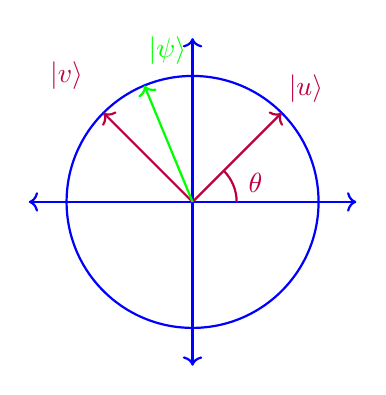
\begin{tikzpicture}[scale=1.6]

% Circle
\draw[thick, blue] (0,0) circle (1);

% Axes with arrow tips
\draw[thick, blue, <->] (-1.3,0) -- (1.3,0);
\draw[thick, blue, <->] (0,-1.3) -- (0,1.3);

\draw[thick, purple, ->] (0,0) -- ({cos(45)},{sin(45)});
\node[purple] at (0.9,0.9) {$\ket{u}$};

\draw[thick, purple, ->] (0,0) -- ({cos(135)},{sin(135)});
\node[purple] at (-1.0,1.0) {$\ket{v}$};

% |psi> vector near vertical axis but slightly right (100 degrees)
\draw[thick, green, ->] (0,0) -- ({cos(112.5)},{sin(112.5)});
\node[green] at (-0.2,1.2) {$\ket{\psi}$};

% Angle theta between horizontal and u
\draw[thick, purple] (0.35,0) arc (0:45:0.35);
\node[purple] at (0.5,0.15) {$\theta$};

\end{tikzpicture}
\end{center}

$$\ket{u} = R_\theta\ket{0}$$
$$\ket{v} = R_\theta\ket{1}$$

For any state:
\begin{align*}
    \ket{\psi} &= \alpha\ket{u} + \beta\ket{v}\\
    &= \alpha \cdot R_\theta\ket{0} + \beta \cdot R_\theta\ket{1}
\end{align*}


\textbf{How to measure in $\ket{u}, \ket{v}$ while actually measuring in standard basis?}

Apply $R_{-\theta}$ to $\ket{\psi}$:
$$R_{-\theta}\ket{\psi} = \alpha\ket{0} + \beta\ket{1}$$

Then measure in $\{\ket{0}, \ket{1}\}$:
\begin{itemize}
\item $\ket{0}$ with probability $|\alpha|^2$ $\rightarrow$ output $\ket{u}$
\item $\ket{1}$ with probability $|\beta|^2$ $\rightarrow$ output $\ket{v}$.
\end{itemize}

\paragraph{Reflections}

\textbf We can also build reflectors along any axis.

\textbf{Example 1:} Reflection along diagonal axis

\begin{center}
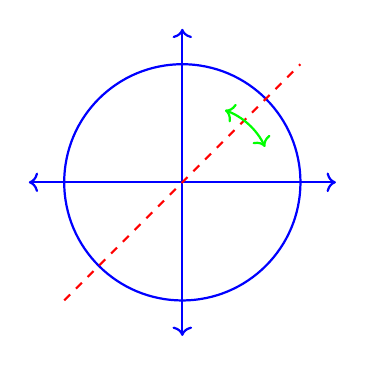
\begin{tikzpicture}[scale=1.5]
% Draw circle
\draw[thick, blue] (0,0) circle (1);
% Draw axes with arrows on both ends
\draw[thick, blue, <->] (-1.3,0) -- (1.3,0);
\draw[thick, blue, <->] (0,-1.3) -- (0,1.3);
% Draw diagonal reflection axis (red dashed)
\draw[thick, red, dashed] (-1,-1) -- (1,1);
% Add green curved arrow showing reflection
\draw[thick, green, <->] (0.7,0.3) arc (25:70:0.6);
\end{tikzpicture}
\end{center}

Reflection transformations:
$$\begin{pmatrix} 1 \\ 0 \end{pmatrix} \to \begin{pmatrix} 0 \\ 1 \end{pmatrix}, \quad \begin{pmatrix} 0 \\ 1 \end{pmatrix} \to \begin{pmatrix} 1 \\ 0 \end{pmatrix}$$
$$\ket{0} \to \ket{1}, \quad \ket{1} \to \ket{0}$$

For a general state:
$$\begin{pmatrix} \alpha \\ \beta \end{pmatrix} \text{ gets transformed to } \begin{pmatrix} \beta \\ \alpha \end{pmatrix}$$

\textbf{NOT operation:} 
$$\ket{\psi} = \begin{pmatrix} \alpha \\ \beta \end{pmatrix} \text{ maps to } \begin{pmatrix} 0 & 1 \\ 1 & 0 \end{pmatrix}\begin{pmatrix} \alpha \\ \beta \end{pmatrix}$$

\textbf{Example 2:} Hadamard gate (reflection along different axis)

\begin{center}
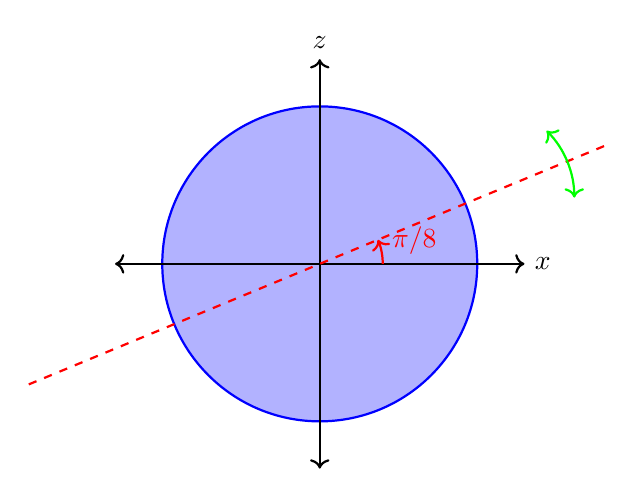
\begin{tikzpicture}[scale=2]
% Draw filled circle
\fill[blue!30] (0,0) circle (1);
\draw[thick, blue] (0,0) circle (1);
% Draw axes with arrows on both ends
\draw[thick, black, <->] (-1.3,0) -- (1.3,0) node[right] {$x$};
\draw[thick, black, <->] (0,-1.3) -- (0,1.3) node[above] {$z$};
% Draw Hadamard reflection axis at pi/8 (22.5 degrees) extended more beyond circle
\draw[thick, red, dashed] ({-2.0*cos(22.5)},{-2.0*sin(22.5)}) -- ({2.0*cos(22.5)},{2.0*sin(22.5)});
% Add green curved arrow centered on the dotted axis at distance 1.1
% Arc from (22.5-22.5) to (22.5+22.5) degrees, radius 0.6, centered at point on axis
\draw[thick, green, <->] ({1.1*cos(22.5)+0.6*cos(0)},{1.1*sin(22.5)+0.6*sin(0)}) arc (0:45:0.6);
% Draw arc showing pi/8 angle from horizontal axis to dashed line
\draw[thick, red, ->] (0.4,0) arc (0:22.5:0.4);
\node[red] at (0.60,0.15) {$\pi/8$};
\end{tikzpicture}
\end{center}

Hadamard transformations:
$$\ket{0} \text{ maps to } \ket{+}$$
$$\ket{1} \text{ maps to } \ket{-}$$

$$\psi = \begin{pmatrix} \alpha \\ \beta \end{pmatrix} \text{ is mapped to } \begin{pmatrix} \frac{1}{\sqrt{2}} & \frac{1}{\sqrt{2}} \\ \frac{1}{\sqrt{2}} & -\frac{1}{\sqrt{2}} \end{pmatrix}\begin{pmatrix} \alpha \\ \beta \end{pmatrix}$$

This is labeled the Hadamard gate and is arguably the most important transformation in quantum computing.

\subsection{Elitzur-Vaidman Revisited}

\textbf{Improved Quantum Strategy via small-angle rotations (Quantum Zeno effect)}
We now show how to make the explosion probability arbitrarily small. Let $\varepsilon = \frac{\pi}{2N}>0$ be a small angle, i.e. $N$ is large. Define the rotation operator
\[
R_\varepsilon=
\begin{pmatrix}
\cos\varepsilon & -\sin\varepsilon\\
\sin\varepsilon & \cos\varepsilon
\end{pmatrix}.
\]
Starting from $\ket{0}$, we perform the following protocol:

\begin{enumerate}
    \item Apply $R_\varepsilon$.
    \item Send the qubit through the unknown box.
    \item If no explosion occurs, repeat the above steps $N$ times.
    \item Finally, measure in the computational basis.
\end{enumerate}

\textbf{Dud:} Since $N=\frac{\pi}{2\varepsilon}$, in the dud case the cumulative rotation is
\[
R_\varepsilon^N = R_{\pi/2},
\]
which maps $\ket{0}$ close to $\ket{1}$. Thus after $N$ rounds the state is approximately $\ket{1}$, and a final measurement yields outcome $\ket{1}$ with full certainty.

\textbf{Working Bomb:} After a single application of $R_\varepsilon$ the state becomes $\cos\varepsilon\ket{0}+\sin\varepsilon\ket{1}$. The box then measures in the computational basis. The probability of explosion in that round is $\sin^2\varepsilon \leq \varepsilon^2$. If no explosion occurs, the state collapses back to $\ket{0}$, and the process repeats.

By the union bound, the probability of at least one explosion over $N$ rounds is upper-bounded by $N\varepsilon^2=\frac{\pi}{2}\varepsilon$, tending to $0$ as $\varepsilon \to 0$. Meanwhile, if no explosion occurs for any of the $N$ rounds, the final measurement yields $\ket{0}$, in stark contrast to the dud case, which yields $\ket{1}$. Thus by choosing $\varepsilon$ sufficiently small, we can distinguish a live bomb from a dud
with arbitrarily high confidence, while making the probability of explosion arbitrarily small.

In a nutshell, using this quantum Zeno strategy we have
\begin{align*}
    \Pr(\text{observe } \ket{1}\,|\,\text{ DUD }) &= 1\\
    \Pr(\text{observe } \ket{0}\,|\,\text{ BOMB }) &\geq 1 - \frac{\pi}{2}\varepsilon.
\end{align*}


\section{Unitary Operations}
We have already seen some operations like the \textbf{NOT} operation and the \textbf{Hadamard} operation. We will now understand what kind of transformations are allowed on quantum states. The transformations that are physically allowed on quantum states are called unitary transformations (or operations). Intuitively, unitaries preserve the `length' of quantum states, thus preserving probability densities.

\textbf{Quantum Mechanics Law 3:} Quantum states can be transformed (without losing information) via \textbf{unitary transformations}.

\begin{definition}[Unitary Matrices]
    A linear transformation $U : \mathcal{H} \to \mathcal{H}$ on a complex Hilbert space is called \textbf{unitary} if it preserves the norm of every state. That is,
    \[
        \| U \ket{\vec{\psi}} \|^2 = \| \ket{\vec{\psi}} \|^2
        \quad \text{for all } \ket{\vec{\psi}} \in \mathcal{H}.
    \]
\end{definition}

Here are a few examples of unitary matrices:
\begin{example}[Examples of Unitary Matrices]\hfill
\begin{enumerate}
\item \textbf{Identity:} $I = \begin{pmatrix} 1 & 0 \\ 0 & 1 \end{pmatrix}$

\item \textbf{Pauli-X (NOT gate):} $X = \begin{pmatrix} 0 & 1 \\ 1 & 0 \end{pmatrix}$

Effect: $X\ket{0} = \ket{1}$ and $X\ket{1} = \ket{0}$ (bit flip)

\item \textbf{Pauli-Y:} $Y = \begin{pmatrix} 0 & -i \\ i & 0 \end{pmatrix}$

\item \textbf{Pauli-Z (phase flip):} $Z = \begin{pmatrix} 1 & 0 \\ 0 & -1 \end{pmatrix}$

Effect: $Z\ket{0} = \ket{0}$ and $Z\ket{1} = -\ket{1}$

\item \textbf{Hadamard gate:} $H = \frac{1}{\sqrt{2}}\begin{pmatrix} 1 & 1 \\ 1 & -1 \end{pmatrix}$

Effect: Creates equal superpositions
\begin{align*}
H\ket{0} &= \frac{1}{\sqrt{2}}(\ket{0} + \ket{1}) = \ket{+} \\
H\ket{1} &= \frac{1}{\sqrt{2}}(\ket{0} - \ket{1}) = \ket{-}
\end{align*}

Note: $H^2 = I$ (Hadamard is self-inverse).

\item \textbf{Phase gate (S gate):} $S = \begin{pmatrix} 1 & 0 \\ 0 & i \end{pmatrix}$

\item \textbf{T gate ($\pi/8$ gate):} $T = \begin{pmatrix} 1 & 0 \\ 0 & e^{i\pi/4} \end{pmatrix}$

\item \textbf{Rotation gates:}
$R_z(\theta) = \begin{pmatrix} e^{-i\theta/2} & 0 \\ 0 & e^{i\theta/2} \end{pmatrix}$
\end{enumerate}
\end{example}






\subsection{Properties of Unitaries}
Let us present the various characterizations of unitary matrices.

\begin{proposition}[Basic Properties of Unitary Matrices]\hfill
\begin{enumerate}
\item \textbf{Preservation of inner products and norms)}: for any $\ket{v}, \ket{w}$:
$\langle Uv | Uw \rangle = \langle v | U^\dagger U | w \rangle = \langle v | w \rangle$. In particular, $\|U\ket{v}\|^2 = \|\ket{v}\|^2$.

\item \textbf{Preservation of angles}: Since $\cos(\theta) := \frac{\langle v | w \rangle}{\|v\|\|w\|}$ and unitary transformations preserve both inner products and norms, the angle between any two vectors is also preserved.

\item \textbf{Eigenvalues lie on unit circle:} If $U\ket{v} = \lambda\ket{v}$, then $|\lambda| = 1$.
\textit{Proof:} $\|\ket{v}\|^2 = \|U\ket{v}\|^2 = \|\lambda\ket{v}\|^2 = |\lambda|^2\|\ket{v}\|^2$, so $|\lambda| = 1$.

\item \textbf{Determinant has unit modulus:} $|\det(U)| = 1$. \textit{Proof:} take determinants on both sides of $U^\dag U=I$.

\item \textbf{Composition of unitaries is unitary:} If $U, V$ are unitary, then $(UV)^\dagger(UV) = V^\dagger U^\dagger U V = V^\dagger V = I$.

\item \textbf{Inverse is unitary:} If $U$ is unitary, so is $U^\dagger = U^{-1}$.

\item \textbf{Reversibility:} Quantum evolution is reversible. Given $\ket{\psi'} = U\ket{\psi}$, we can always recover $\ket{\psi} = U^{-1}\ket{\psi'}= U^\dagger\ket{\psi'}$.

\item \textbf{Square roots exist:} Every unitary $U$ has a square root $W$, which is also unitary, such that $W^2 = U$. This allows for fractional quantum operations.

\textit{Example:} Consider the NOT gate (Pauli-X): $X = \begin{pmatrix} 0 & 1 \\ 1 & 0 \end{pmatrix}$. Its square root is:
$$\sqrt{X} = \frac{1}{2}\begin{pmatrix} 1+i & 1-i \\ 1-i & 1+i \end{pmatrix}$$

We can verify: $\sqrt{X} \cdot \sqrt{X} = \frac{1}{4}\begin{pmatrix} 1+i & 1-i \\ 1-i & 1+i \end{pmatrix}\begin{pmatrix} 1+i & 1-i \\ 1-i & 1+i \end{pmatrix} = \begin{pmatrix} 0 & 1 \\ 1 & 0 \end{pmatrix} = X$

On the Bloch sphere, $\sqrt{X}$ represents a rotation halfway to the full NOT operation.
\end{enumerate}
\end{proposition}


\subsection{Classical Analogue of Unitary Transformations}
It is instructive to compare unitary evolution in quantum mechanics with the way probability distributions evolve in classical randomized processes. In the classical setting, a system with $d$ possible outcomes can be represented by a probability vector
\[
p =
\begin{bmatrix}
p_1\\
p_2\\
\vdots\\
p_d
\end{bmatrix},
\qquad
p_i \ge 0,
\qquad
\sum_{i=1}^d p_i = 1.
\]

A randomized procedure transforms $p$ into a new distribution $p'$ via multiplication by a matrix $M$:
\[
p' = Mp.
\]
To preserve total probability, such a matrix must be column-stochastic, meaning its entries are non-negative and each column sums to $1$:
\[
M_{ij}\ge 0
\qquad\text{and}\qquad
\sum_{i=1}^d M_{ij} = 1 \ \ \text{for all } j.
\]

We now illustrate this with a classical example.

Consider the following random process: we roll a fair die; if the outcome is odd, we toss a fair coin; if it's heads, add $1$ to the outcome of the fair die.

Let the state space be $\{1,2,3,4,5,6\}$, and start from the uniform distribution
\[
p=
\begin{bmatrix}
\frac16\\
\frac16\\
\frac16\\
\frac16\\
\frac16\\
\frac16
\end{bmatrix}.
\]
The transformation implemented by the above procedure is captured by the column-stochastic matrix
\[
M=
\begin{bmatrix}
\frac12 & 0 & 0 & 0 & 0 & 0\\
\frac12 & 1 & 0 & 0 & 0 & 0\\
0 & 0 & \frac12 & 0 & 0 & 0\\
0 & 0 & \frac12 & 1 & 0 & 0\\
0 & 0 & 0 & 0 & \frac12 & 0\\
0 & 0 & 0 & 0 & \frac12 & 1
\end{bmatrix},
\qquad
p' = Mp.
\]
Starting from an odd face $1,3,5$, the coin toss either keeps the value (tails) or moves it to the next even face (heads), giving the $\frac12$--$\frac12$ split in the corresponding column. Starting from an even face $2,4,6$, the value stays unchanged, which is why the corresponding column has a single $1$.

This classical picture is quite similar to quantum evolution in that both are linear transformations on vectors. However, there are key differences.

First, classical stochastic evolution preserves the $\ell_1$ norm,
\[
\|p'\|_1 = \|p\|_1 = 1,
\]
whereas quantum evolution preserves the $\ell_2$ norm,
\[
\|U\ket{\psi}\|_2 = \|\ket{\psi}\|_2.
\]

Second, classical stochastic transformations are generally not reversible: a column-stochastic matrix need not be invertible, and even when it is invertible, its inverse typically does not have non-negative entries and therefore does not correspond to a valid stochastic process. In contrast, every unitary matrix is reversible, with inverse $U^\dagger$ as seen in the characterisation. This reversibility is one of the fundamental distinctions between classical and quantum dynamics.





\newpage

\noindent
\textbf{CS4268 AY2025-26 Sem 2}
\\
\noindent
Lecturer: Divesh Aggarwal
\hfill
Lecture 3                      %%% FILL IN LECTURE NUMBER HERE
\hfill
Date: January 29, 2026          %%% FILL IN LECTURE DATE HERE


\noindent
\rule{\textwidth}{1pt}

\medskip

\section{Composite Systems}
We have discussed how to describe a single quantum system via the notion of quantum states residing in a Hilbert space, how they can be transformed and how information is extracted from the system via measurements. Now we discuss how to characterize \textit{composite} systems. Given two (or more) quantum systems, each with its own Hilbert space, how do we describe them collectively as a whole? In particular, if we only effect changes on a component of this composite system, how can we describe this mathematically as an operation on the entire system? 

This is achieved via the notion of \textit{tensor products}.

\subsection{Tensor Products}
Let us consider a system comprising simply two qudits. This system is mathematically described by the tensor product of the Hilbert spaces of the individual qudits:

\begin{definition}[Tensor Product of Hilbert Spaces]\label{definition:tensor_products}
    Given two qudit Hilbert spaces $\mathcal{H}_1 = \mathbb{C}^{d_1}$, $\mathcal{H}_2 = \mathbb{C}^{d_2}$ spanned respectively by the computational basis vectors
    \[
    \mathcal{B}_1 = \{\ket{0}, \ket{1}, \dots, \ket{d_1-1}\}, \quad 
    \mathcal{B}_2 = \{\ket{0}, \ket{1}, \dots, \ket{d_2-1}\},
    \]
    the \textbf{tensor product} of $\mathcal{H}_1$ and $\mathcal{H}_2$ is defined as the Hilbert space
    \[
    \mathcal{H}_1 \otimes \mathcal{H}_2 = \text{span} \{\ket{i} \otimes \ket{j} : 0 \le i \le d_1-1, 0 \le j \le d_2-1 \}.
    \]

    Each (normalized) state $\ket{\psi} = \sum_{ij} {a_{ij}}\ket{i} \otimes \ket{j} \in \mathcal{H}_1 \otimes \mathcal{H}_2$, $\sum_{ij}|a_{ij}|^2=1$, is a legitimate characterization of the entire system. Also, for brevity we shall henceforth write $\ket{\alpha} \otimes \ket{\beta}$ simply as $\ket{\alpha\beta}$.

    More generally, for $n>2$ systems, the tensor product generalizes naturally to
    \[
    \mathcal{H}_1 \otimes \mathcal{H}_2 \otimes \dots \otimes \mathcal{H}_n = \text{span}\{\ket{i_1}\otimes \dots \otimes \ket{i_n}\}.
    \]
\end{definition}

\begin{remark}[Existence and Uniqueness of Tensor Products]
    Note that above we have defined the tensor product as being the span of the \textit{formal} symbols $\ket{i} \otimes \ket{j}$ -- we have not at all dissected what the symbols $\ket{i} \otimes \ket{j}$ really mean. In particular, what is the difference between $\ket{i} \otimes \ket{j}$ and the \textit{direct sum} $(\ket{i}, \ket{j})$? Superficially, both seem quite similar in the sense that the individual constituents are simply concatenated together (albeit in different notations). Indeed, these two notions are closely related: roughly speaking, we think of the symbol $\otimes$ as a \textit{bilinear map} from the direct sum/Cartesian product $H_1 \times H_2$ to the Hilbert space $Z$ (we use the symbol $Z$ because we have not yet proved that this thing exists). That is, the purported map $\otimes$ behaves as such (on all vectors $\ket{u}, \ket{v}$, not just the basis vectors):
    \begin{align*}
        \otimes(\ket{u},\ket{v}) := \ket{u} \otimes \ket{v}
    \end{align*}
    such that
    \begin{align}\label{equation:tensor_product_multilinearity}
        (a\ket{u_1}+b\ket{u_2}) \otimes \ket{v} &= a\ket{u_1} \otimes \ket{v} + b\ket{u_2} \otimes \ket{v}\\
        \ket{u} \otimes(a\ket{v_1}+b\ket{v_2}) &= a\ket{u} \otimes \ket{v_1} + b\ket{u} \otimes \ket{v_2}.
    \end{align}
    The existence and (essential) uniqueness of the map $\otimes$ is nontrivial to show. Once these are taken care of we can start calling $Z$ as $H_1 \otimes H_2$. If you are interested, the wiki article on \href{https://en.wikipedia.org/wiki/Tensor_product}{tensor products} is a good starting point. Be warned however that this leads to a long rabbit hole.

    That was a lot of yapping -- but we won't worry about any of that in this course. In practice, think of $\otimes$ as concatenation plus multilinearity: the symbol $\otimes$ is used to stack different basis vectors from different Hilbert spaces together, and that $\otimes$ is linear with respect to \textit{all} its arguments, i.e. \cref{equation:tensor_product_multilinearity}
\end{remark}

\begin{fact}[Column Vector Representation of Tensor Products]
    Given vectors $\ket{\alpha} \in \mathcal{H}_1$ and $\ket{\beta} \in \mathcal{H}_2$, the column representation of $\ket{\alpha}\otimes \ket{\beta}$ is given by
    \begin{align*}
        \ket{a} \otimes \ket{b} = \begin{pmatrix} a_0 \\ \vdots \\ a_{d_1-1} \end{pmatrix} \otimes \begin{pmatrix} b_0 \\ \vdots \\ b_{d_2-1} \end{pmatrix} = \begin{pmatrix} a_0 b_0 \\ \vdots \\ a_0 b_{d_2-1} \\ \vdots \\ a_{d_1-1} b_{0} \\ \vdots \\ a_{d_1-1} b_{d_2-1} \end{pmatrix}.
    \end{align*}
    In particular, the tensor product of the basis vectors is given by
    \[
    \ket{i} \otimes \ket{j} =
    \begin{bmatrix}0 \\ \vdots \\ 1 \\ \vdots \\ 0 \end{bmatrix}
    \]
    where the $1$ appears at position $i \cdot d_2 + j$.
\end{fact}
These results are immediate from the definition of the tensor product.

\begin{example}
    For two qubits ($d_1 = d_2 = 2$), the computational basis states are represented as
    \[
    \ket{0} = \begin{bmatrix}1\\0\end{bmatrix}, \qquad
    \ket{1} = \begin{bmatrix}0\\1\end{bmatrix}.
    \]
    The superposition states are
    \[
    \ket{+} = \frac{1}{\sqrt{2}}\begin{bmatrix}1\\1\end{bmatrix}, \qquad
    \ket{-} = \frac{1}{\sqrt{2}}\begin{bmatrix}1\\-1\end{bmatrix}.
    \]
    
    We now give examples of tensor products in column-vector form:
    \begin{align*}
    \ket{0}\otimes\ket{0}
    &=
    \begin{bmatrix}1\\0\\0\\0\end{bmatrix},\\[6pt]
    \ket{0}\otimes\ket{+}
    &=
    \frac{1}{\sqrt{2}}
    \begin{bmatrix}1\\1\\0\\0\end{bmatrix},\\[6pt]
    \ket{+}\otimes\ket{0}
    &=
    \frac{1}{\sqrt{2}}
    \begin{bmatrix}1\\0\\1\\0\end{bmatrix},\\[6pt]
    \ket{+}\otimes\ket{-}
    &=
    \frac{1}{2}
    \begin{bmatrix}1\\-1\\1\\-1\end{bmatrix}.
    \end{align*}

    More generally, suppose Alice has qubit $\ket{A} = \alpha_0\ket{0} + \alpha_1\ket{1}$ and Bob has qubit $\ket{B} = \beta_0\ket{0} + \beta_1\ket{1}$. Then their joint state is
    \[
    \ket{A}\otimes\ket{B} = \alpha_0\beta_0 \ket{0}\otimes\ket{0} + \alpha_0\beta_1 \ket{0}\otimes\ket{1} 
    + \alpha_1\beta_0 \ket{1}\otimes\ket{0} + \alpha_1\beta_1 \ket{1}\otimes\ket{1}.
    \]
    Notice how the multilinearity (bilinearity here) was invoked to obtain this expansion. In column vector form:
    \[
    \ket{A}\otimes\ket{B} =
    \begin{bmatrix}
    \alpha_0\beta_0 \\ \alpha_0\beta_1 \\ \alpha_1\beta_0 \\ \alpha_1\beta_1
    \end{bmatrix}.
    \]
    To verify that the composite coefficients are indeed probability amplitudes, we check if the sum of amplitudes squared is 1. But this is easy -- according to Quantum Mechanics Law 1, the amplitudes of $\ket{A}$ and $\ket{B}$ satisfy the \textbf{normalization condition} i.e. $|\alpha_0|^2 + |\alpha_1|^2 = 1$ and $|\beta_0|^2 + |\beta_1|^2 = 1$, so
    \begin{align*}
    |\alpha_0\beta_0|^2 + |\alpha_0\beta_1|^2 + |\alpha_1\beta_0|^2 + |\alpha_1\beta_1|^2
    &= |\alpha_0|^2(|\beta_0|^2 + |\beta_1|^2) + |\alpha_1|^2(|\beta_0|^2 + |\beta_1|^2)\\
    &= |\alpha_0|^2 + |\alpha_1|^2\\
    &= 1
    \end{align*}
    as desired.
\end{example}

\begin{definition}[Tensor Product of Matrices]
    Given matrices $A \in \mathbb{C}^{m\times n}$ and $B \in \mathbb{C}^{p\times q}$, their tensor (also called Kronecker) product $A \otimes B$ is the $mp \times nq$ matrix
    \[
    A \otimes B =
    \begin{bmatrix}
    a_{11}B & a_{12}B & \cdots & a_{1n}B \\
    a_{21}B & a_{22}B & \cdots & a_{2n}B \\
    \vdots & \vdots & \ddots & \vdots \\
    a_{m1}B & a_{m2}B & \cdots & a_{mn}B
    \end{bmatrix}.
    \]
\end{definition}

\begin{remark}
    We seem to have two different (but superficially very similar) notions of tensor products, one for vectors and one for matrices, but note that technically the set of matrices itself is an abstract vector space, thus there really is no difference on an abstract level. The only difference here of course is the \textit{concrete representation} of the objects. What we call vectors in this course we generally write down as columns (long-ish 1D objects), while the operators on these vectors (which technically speaking also form a vector space themselves) we write down as matrices (square-ish 2D objects). Hopefully this isn't too confusing. If it helps you can restack the rectangular-looking matrices into long columns (vectorization). Then the basis matrices spanning matrix space gets rewritten as long, all-zeros-except-one vectors. Then this should be very clear that the tensor product of matrices is exactly the same as the general definition given in \cref{definition:tensor_products}.
\end{remark}
 

\begin{proposition}
The tensor product of matrices satisfies the following properties:
\begin{itemize}
    \item $(A \otimes B)(C \otimes D) = (AC) \otimes (BD)$ whenever dimensions match.
    \item $(A \otimes B)^\dagger = A^\dagger \otimes B^\dagger$.
    \item $\mathrm{Tr}(A \otimes B) = \mathrm{Tr}(A)\mathrm{Tr}(B)$.
    \item If $A$ and $B$ are invertible, then $(A \otimes B)^{-1} = A^{-1} \otimes B^{-1}$.
\end{itemize}
\end{proposition}

Why are matrix tensor products useful? Recall that matrices appear a lot in quantum, as operations on the quantum states (unitaries, measurements etc). Matrix tensor products characterize the \textit{joint} application of these operations on the entire system. Consider a two qubit basis state $\ket{\psi}=\ket{00}$. Suppose we apply a unitary transformation $U= \begin{bmatrix} p & r \\ q & s \end{bmatrix}$ only to the second qubit.

The overall transformation on $\ket{\psi}$ can be described by
$$
    \ket{00} \rightarrow \ket{0} \otimes (U\ket{0})
$$
The transformations for the other basis states can be obtained similarly. Specifically:
\begin{align*}
    \ket{00} &\rightarrow \ket{0} \otimes (U\ket{0}) = \begin{bmatrix}
        p \\ q \\ 0 \\ 0
    \end{bmatrix} \\
    \ket{01} &\rightarrow \ket{0} \otimes (U\ket{1}) = \begin{bmatrix}
        r \\ s \\ 0 \\ 0
    \end{bmatrix} \\
    \ket{10} &\rightarrow \ket{1} \otimes (U\ket{0}) = \begin{bmatrix}
        0 \\ 0 \\ p \\ q
    \end{bmatrix} \\
    \ket{11} &\rightarrow \ket{1} \otimes (U\ket{1}) = \begin{bmatrix}
        0 \\ 0 \\ r \\s
    \end{bmatrix}.
\end{align*}
Denoting $I$ as the identity matrix, this transformation can be succinctly written as
$$
    I \otimes U \ket{\psi}
$$
where
\begin{align*}
    I \otimes U &= \begin{bmatrix}
        p & r & 0 & 0 \\
        q & s & 0 & 0 \\
        0 & 0 & p & r \\
        0 & 0 & q & s
    \end{bmatrix}
\end{align*}
Intuitively, the `do nothing' operation on the first qubit is mathematically represented as applying the identty operator on the first qubit.

\begin{theorem}[Single Qubit Unitary Transformations in Composite System]
Suppose $U, V$ are unitary transformations.
If we apply $U$ to $\ket{\phi}$ and $V$ to $\ket{\psi}$, the joint state $\ket{\phi\psi}$ is transformed to $U \otimes V \ket{\phi\psi}$.
\end{theorem}

\begin{proof}
    We can consider the unitary transformations applied to $\ket{\phi}$ and $\ket{\psi}$ as two separate unitary transformations applied consecutively:
    \begin{align*}
        (I \otimes V)(U \otimes I) \ket{\phi\psi} &= (IU) \otimes (VI) \ket{\phi\psi} \quad ((A \otimes B)(C \otimes D) = (AC) \otimes (BD)) \\
        &= (U \otimes V) \ket{\phi\psi}.
    \end{align*}
\end{proof}

Next we consider an extremely important gate in quantum computing, the \textbf{CNOT gate}. A CNOT gate takes in two qubits, a control qubit and a target qubit.
Denote the control qubit as $\ket{\phi}$ and the target qubit as $\ket{\psi}$.
\begin{itemize}
    \item If the control qubit is $0$, do nothing.
    \item If the control qubit is $1$, flip the target qubit.
\end{itemize}
Given $\ket{\phi\psi}$, enumerating over all the basis states, we have the following transformations effected by CNOT:
\begin{align*}
    \ket{00} &\rightarrow \ket{00} \\
    \ket{01} &\rightarrow \ket{01} \\
    \ket{10} &\rightarrow \ket{11} \\
    \ket{11} &\rightarrow \ket{10}.
\end{align*}
Note that the resulting basis is still orthonormal. The CNOT gate can be represented by the following matrix,
\begin{align*}
    \text{CNOT} &= \begin{bmatrix}
        1 & 0 & 0 & 0 \\
        0 & 1 & 0 & 0 \\
        0 & 0 & 0 & 1 \\
        0 & 0 & 1 & 0
    \end{bmatrix}.
\end{align*}
The first two columns in the CNOT matrix represents the transformation to $\ket{\psi}$ when $\phi = 0$,
while the last two columns in the CNOT matrix represents the ``flipping'' transformation to $\ket{\psi}$ when $\phi = 1$.

The probability amplitudes of the original basis will be mapped to the corresponding basis after the CNOT operation. More concretely,
\begin{align*}
    \begin{bmatrix}
        1 & 0 & 0 & 0 \\
        0 & 1 & 0 & 0 \\
        0 & 0 & 0 & 1 \\
        0 & 0 & 1 & 0
    \end{bmatrix} \begin{bmatrix}
        \alpha_{00} \\ \alpha_{01} \\ \alpha_{10} \\ \alpha_{11}
    \end{bmatrix} &= \begin{bmatrix}
        \alpha_{00} \\ \alpha_{01} \\ \alpha_{11} \\ \alpha_{10}
    \end{bmatrix}.
\end{align*}

CNOT as a diagram:
\begin{center}
    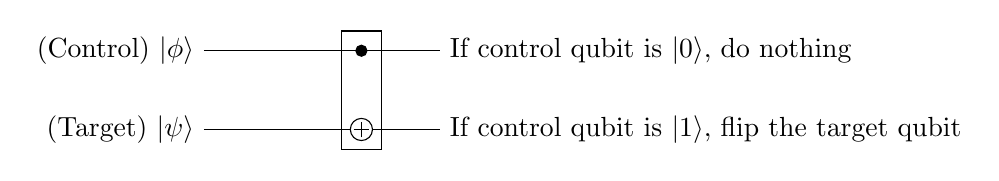
\begin{tikzpicture}
    
    \node [left] at (0, 1) {(Control) $\ket{\phi}$};
    \node [right] at (3, 1) {If control qubit is $\ket{0}$, do nothing};
    \node [left] at (0, 0) {(Target) $\ket{\psi}$};
    \node [right] at (3, 0) {If control qubit is $\ket{1}$, flip the target qubit};
    
    \draw (0, 1) -- (3, 1);
    \draw (0, 0) -- (3, 0);
    
    \filldraw [black] (2, 1) circle (2pt);
    \filldraw [draw=black, fill=white] (2, 0) circle (4pt);
    
    \draw (1.9, 0) -- (2.1, 0);
    \draw (2, -0.1) -- (2, 0.1);
    
    \draw (1.75, 1.25) -- (2.25, 1.25) -- (2.25, -0.25) -- (1.75, -0.25) -- cycle;
    
    \end{tikzpicture}
\end{center}

The next example on creating EPR states is intended to be a hands-on exercise to help you gain familiarity with tensor product manipulation.

\begin{example}[Creating EPR/Bell states]
To produce the EPR state $\ket{\Phi^+}:= \frac{1}{\sqrt{2}}(\ket{00} + \ket{11})$, we use a circuit consisting of a Hadamard gate ($H$) followed by a CNOT:
\begin{enumerate}
    \item \textbf{Initial State:} $\ket{\psi_0} = \ket{0} \otimes \ket{0} = \ket{00}$.
    \item \textbf{Apply $H$ to first qubit:} $\ket{\psi_1} = (H \otimes I)\ket{00} = \left(\frac{\ket{0} + \ket{1}}{\sqrt{2}}\right) \otimes \ket{0} = \frac{1}{\sqrt{2}}(\ket{00} + \ket{10})$.
    \item \textbf{Apply CNOT:} $\ket{\psi_2} = \text{CNOT} \left( \frac{1}{\sqrt{2}}(\ket{00} + \ket{10}) \right) = \frac{1}{\sqrt{2}}(\ket{00} + \ket{11})$.
\end{enumerate}

Diagrammatically,
    \begin{center}
        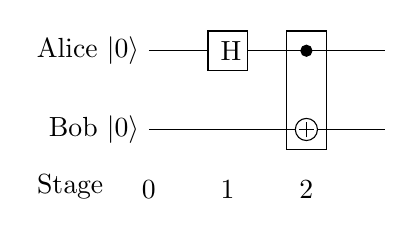
\begin{tikzpicture}
        
        \node [left] at (0, 1) {Alice $\ket{0}$};
        \node [left] at (0, 0) {Bob $\ket{0}$};

        \node [above] at (-1, -1) {Stage};
        \node [above] at (0, -1) {0};
        \node [above] at (1, -1) {1};
        \node [above] at (2, -1) {2};
        
        \draw (0, 1) -- (3, 1);
        \draw (0, 0) -- (3, 0);
        
        \filldraw [black] (2, 1) circle (2pt);
        \filldraw [draw=black, fill=white] (2, 0) circle (4pt);
        
        \draw (1.9, 0) -- (2.1, 0);
        \draw (2, -0.1) -- (2, 0.1);

        % H gate
        \draw [fill=white] (0.75, 1.25) -- (1.25, 1.25) -- (1.25, 0.75) -- (0.75, 0.75) -- cycle;
        \node [left] at (1.3, 1) {H};
        
        \draw (1.75, 1.25) -- (2.25, 1.25) -- (2.25, -0.25) -- (1.75, -0.25) -- cycle;
        
        \end{tikzpicture}
    \end{center}
\end{example}

\subsection{Quantum Entanglement}
Look at the Bell state again. We might think: what is the appropriate $\ket{\psi}$ and $\ket{\phi}$ such that $\ket{\Phi^+} = \ket{\psi} \otimes \ket{\phi}$? That is, what are the individual states of the qubits that collectively are described as the Bell state $\ket{\Phi^+}$ on the entire system?

Answer: there are no pairs of individual states $\ket{\phi}$ and $\ket{\psi}$ such that $\ket{\Phi^+} = \ket{\phi} \otimes \ket{\psi}$.
\begin{proof}
Assume that $\ket{\Phi^+} = \frac{1}{\sqrt{2}}(\ket{00} + \ket{11})$ is separable, i.e. there exist states $\ket{\psi} = \alpha_0\ket{0} + \alpha_1\ket{1}$ and $\ket{\phi} = \beta_0\ket{0} + \beta_1\ket{1}$ such that $$\ket{\Phi^+} = \ket{\psi} \otimes \ket{\phi}.$$

Expanding the tensor product out gives
\begin{align*}
\ket{\psi} \otimes \ket{\phi} &= (\alpha_0\ket{0} + \alpha_1\ket{1}) \otimes (\beta_0\ket{0} + \beta_1\ket{1}) \\
&= \alpha_0\beta_0\ket{00} + \alpha_0\beta_1\ket{01} + \alpha_1\beta_0\ket{10} + \alpha_1\beta_1\ket{11}
\end{align*}

We compare the coefficients of this expansion to the Bell state $\frac{1}{\sqrt{2}}\ket{00} + 0\ket{01} + 0\ket{10} + \frac{1}{\sqrt{2}}\ket{11}$:
\begin{enumerate}
    \item $\alpha_0\beta_0 = \frac{1}{\sqrt{2}}$ (from $\ket{00}$)
    \item $\alpha_0\beta_1 = 0$ (from $\ket{01}$)
    \item $\alpha_1\beta_0 = 0$ (from $\ket{10}$)
    \item $\alpha_1\beta_1 = \frac{1}{\sqrt{2}}$ (from $\ket{11}$)
\end{enumerate}

From (2), either $\alpha_0 = 0$ or $\beta_1 = 0$.
\begin{itemize}
    \item If $\alpha_0 = 0$, then $\alpha_0\beta_0 = 0$, which contradicts (1).
    \item If $\beta_1 = 0$, then $\alpha_1\beta_1 = 0$, which contradicts (4).
\end{itemize}

Since both possibilities lead to a contradiction, no such $\alpha_i, \beta_i$ exist. Therefore, $\ket{\Phi^+}$ is nonseparable.
\end{proof}

We say that $\ket{\Phi^+}$ is an \textbf{entangled} state. (Quantum) Entanglement is a \textit{core} feature of quantum mechanics and quantum computing, but mathematically it simply expresses the non-separability of the system state.

\begin{definition}[Separability and Entanglement]
Consider a composite quantum system described by the Hilbert space $\mathcal{H} = \mathcal{H}_A \otimes \mathcal{H}_B$. 
\begin{itemize}
    \item A pure state $\ket{\Psi} \in \mathcal{H}$ is said to be \textbf{separable} (or non-entangled) if it can be written as a tensor product of states from the individual subsystems:
    $$\ket{\Psi} = \ket{\psi}_A \otimes \ket{\phi}_B$$
    where $\ket{\psi}_A \in \mathcal{H}_A$ and $\ket{\phi}_B \in \mathcal{H}_B$.
    
    \item A pure state $\ket{\Psi}$ is said to be \textbf{entangled} if it cannot be decomposed in such a manner. That is:
    $$\ket{\Psi} \neq \ket{\psi}_A \otimes \ket{\phi}_B \quad \forall \ket{\psi}_A, \ket{\phi}_B$$
\end{itemize}
\end{definition}

While an entangled system state cannot be written as a tensor product of subsystem states, we \textit{can} actually make sense of and talk about these subsystem states, via the concept of partial trace. More on that later in the course.

\subsection{Partial Measurements}

So far we have seen how to describe composite systems and the operations on them, generally speaking. Performing measurements is also a type of operation. In this section we briefly explore the notion of partial measurements, i.e. making measurements only on a subsystem of the whole system.

Intuitively, if Alice measures \emph{only her qubit} in a joint state, she should obtain a classical outcome (here $0$ or $1$) according to the Born rule, and the \emph{post-measurement joint state} should be the part of the superposition consistent with that outcome, renormalized to have norm $1$.

Consider a general two-qubit state (Alice is the first qubit, Bob is the second):
\[
    \ket{\psi}
    = \alpha_{00}\ket{00}+\alpha_{01}\ket{01}+\alpha_{10}\ket{10}+\alpha_{11}\ket{11},
    \qquad
    \sum_{i,j\in\{0,1\}}|\alpha_{ij}|^2=1.
\]
Alice measures her qubit (in the computational basis). We have the case
\[
    \Pr[\text{Alice reads }\ket{0}] = |\alpha_{00}|^2 + |\alpha_{01}|^2
\]
wherein the state collapses to
\[
    \frac{\alpha_{00}\ket{00}+\alpha_{01}\ket{01}}{\sqrt{|\alpha_{00}|^2+|\alpha_{01}|^2}}
    = \gamma_0\ket{00}+\gamma_1\ket{01},
\]
where
\[
    \gamma_0=\frac{\alpha_{00}}{\sqrt{|\alpha_{00}|^2+|\alpha_{01}|^2}},
    \qquad
    \gamma_1=\frac{\alpha_{01}}{\sqrt{|\alpha_{00}|^2+|\alpha_{01}|^2}};
\]
and the case
\[
    \Pr[\text{Alice reads }\ket{1}] = |\alpha_{10}|^2 + |\alpha_{11}|^2
\]
wherein the state collapses to
\[
    \frac{\alpha_{10}\ket{10}+\alpha_{11}\ket{11}}{\sqrt{|\alpha_{10}|^2+|\alpha_{11}|^2}}
    = \gamma_0'\ket{10}+\gamma_1'\ket{11},
\]
where
\[
    \gamma_0'=\frac{\alpha_{10}}{\sqrt{|\alpha_{10}|^2+|\alpha_{11}|^2}},
    \qquad
    \gamma_1'=\frac{\alpha_{11}}{\sqrt{|\alpha_{10}|^2+|\alpha_{11}|^2}}.
\]
The amplitudes $\gamma_0,\gamma_1$ (respectively $\gamma_0',\gamma_1'$) are the \emph{conditional} probability amplitudes of the two-qubit basis states given Alice's outcome. Equivalently, they describe Bob's post-measurement state conditioned on Alice:
\[
    \ket{\psi_B \mid A=0}=\gamma_0\ket{0}+\gamma_1\ket{1},
    \qquad
    \ket{\psi_B \mid A=1}=\gamma_0'\ket{0}+\gamma_1'\ket{1},
\]
since in the $A=0$ branch the joint state is $\ket{0}\otimes(\gamma_0\ket{0}+\gamma_1\ket{1})$, and similarly for $A=1$.

Physically, Alice's measurement \emph{projects} the joint state onto the subspace consistent with her observed classical bit and the renormalization ensures the remaining state has total probability $1$. If $\ket{\psi}$ is a product state, measuring Alice does not change Bob's qubit. If $\ket{\psi}$ is entangled, then Bob's conditional state can depend on Alice's outcome, which is the source of the strong correlations observed in entangled measurements.


\newpage

\noindent
\textbf{CS4268 AY2025-26 Sem 2}
\\
\noindent
Lecturer: Divesh Aggarwal
\hfill
Lecture 4                      %%% FILL IN LECTURE NUMBER HERE
\hfill
Date: February 5, 2026          %%% FILL IN LECTURE DATE HERE


\noindent
\rule{\textwidth}{1pt}

\medskip

\section{The No-Cloning Theorem and Quantum Teleportation}
Every single week during the lecture, a few of you open this overleaf file and copy the scribe template over to your own file to work on it. Some of you use ChatGPT to help refine your scribes (which is okay, just be honest with it). The numerous ctrl-C's/ctrl-V's involved in these undertakings were in all likelihood barely noticed. But they of course were instances of copying/cloning (classical) information, which is ubiquitous. Unfortunately, the same cannot be done with \textit{quantum} information.

\subsection{No Quantum Clones}

\begin{theorem}
    There does not exist a unitary $U$ which upon arbitrary input states $\ket{\psi}$ outputs $\ket{\psi}\ket{\psi}$. More precisely, a unitary such that
    \begin{align*}
        U\ket{\psi}\ket{\text{anc}} = \ket{\psi}\ket{\psi} \quad\forall \ket{\psi}
    \end{align*}
    does not exist. Here $\ket{\text{anc}}$ denotes \textit{any arbitrary} ancillary state which has the same dimension as $\ket{\psi}$.
\end{theorem}
\begin{proof}
    We present two proofs.
    
    Proof 1: Suppose there exists such a unitary $U$. Pick an arbitrary state $\ket{\psi}=a\ket{0}+b\ket{1}$ where $a,b$ are complex amplitudes. Running $U$ on $\ket{\psi}$ yields
    \begin{align*}
        U(a\ket{0}+b\ket{1})\ket{\text{anc}} = a^2\ket{00}+ab\ket{01}+ab\ket{10}+b^2\ket{11}.
    \end{align*}
    But at the same time we also have $U\ket{0}\ket{\text{anc}}=\ket{00}$ and $U\ket{1}\ket{\text{anc}}=\ket{11}$. By linearity we thus have 
    \begin{align*}
        U(a\ket{0}+b\ket{1})\ket{\text{anc}} = a\ket{00}+b\ket{11}.
    \end{align*}
    Matching the two given expressions for $U\ket{\psi}\ket{\text{anc}}$ we see that they are compatible only when $(a,b)=(0,1)$ or $(1,0)$, contradicting the arbitrariness of $\ket{\psi}$.

    Proof 2: Pick two arbitrary states $\ket{\psi}, \ket{\phi}$ and run $U$ on them. This gives $U\ket{\psi}\ket{\text{anc}} = \ket{\psi}\ket{\psi}$ and $U\ket{\phi}\ket{\text{anc}} = \ket{\phi}\ket{\phi}$. Taking their inner products and noting the unitarity of $U$ we see that $\langle \psi|\phi \rangle = \langle \psi|\phi \rangle^2 \implies \langle \psi|\phi \rangle=0/1$. That is, the two states must either be the same or mutually orthogonal, once again contradicting the assumed arbitrariness.
\end{proof}

\subsection{Quantum Teleportation}

Consider the following scenario: suppose we have 2 friends, Alice and Bob, and they live far away from one another. Alice has in her possession some unknown qubit \(\ket{\psi} := \alpha \ket{0} + \beta \ket{1}\) and she wants to send it to Bob. How can she do it? 

\paragraph{A Preliminary Puzzle}
 Before we start off showing how it can be done, let us start off with a simpler puzzle. Suppose Alice and Bob are sitting in the lab, and Alice wants to send some unknown qubit \(\ket{\psi}\) to Bob. Obviously, she cannot walk up to Bob to give it to him but what they do have is a shared network for both of them to perform unitary operations (see \Cref{fig:unknown_quantum_teleporter}).

 \begin{figure}[!ht]
    \centering
    \begin{quantikz}
    \lstick[2]{$\substack{\ket{\psi} := \alpha \ket{0} + \beta \ket{1}\\\\\otimes \\\\\ket
    0}$} & \gate[2]{?} & \rstick[2]{$\substack{\ket{\cdot}\\\\\otimes \\\\\ket
    \psi}$}\\
     & & 
    \end{quantikz}
    \caption{Some unknown quantum teleporter}
    \label{fig:unknown_quantum_teleporter}
\end{figure}

Note that from \Cref{fig:unknown_quantum_teleporter}, we want these states to be un-entangled so that Alice cannot ``destroy" the qubit via a measurement.

What Alice can do is to apply a CNOT operation with a control qubit \(\ket{0}\) followed by a Hadamard operation as follows in \Cref{fig:cnot_hadamard}:

\begin{figure}[!ht]
    \centering
    \begin{quantikz}
    \lstick{\(\alpha\ket{0} + \beta\ket{1}\)} & \ctrl{1} \slice{t=1}& \gate[1]{H} \slice{t=2} &\\
    \lstick{\(\ket{0}\)} & \targ{} & &
    \end{quantikz}
    \caption{Alice's CNOT and Hadamard Operation}
    \label{fig:cnot_hadamard}
\end{figure}

The intuition here is this: suppose Alice measures her qubit, the quantum state of the qubit is going to collapse to \(\ket{0}\) or \(\ket{1}\), which is clearly not what we want. By introducing the CNOT gate, the state is now entangled. One can realise that neither qubit in the entangled state contains the full information of the original qubit. Therefore at \(t = 1\), the state of the quantum system, \(\ket{\psi_1}\) is: \begin{equation}
    \ket{\psi_1} = (\alpha \ket{0} + \beta \ket{1}) \otimes \ket{0} = \alpha \ket{00} + \beta\ket{11}
\end{equation}

Now, we want to remove the entanglement of the quantum state. Alice \textit{could have} measured her qubit but that is not going to be helpful because with probability \(|\alpha|^2\), her qubit is going to be \(\ket{0}\) but then due to the entanglement, Bob's qubit is going to be \(\ket{0}\) with the same probability. The same explanation applies for the state \(\ket{1}\) with probability \(|\beta|^2\). Applying the Hadamard operation on \text{only Alice's qubit} can remove that entanglement. We can see that at \(t = 2\), the state of the quantum system \(\ket{\psi_2}\) is \begin{equation}
    \begin{aligned}
        \ket{\psi_1} &\rightarrow \ket{\psi_2}\\
        &= \alpha \ket{+0} + \beta \ket{-1}\\
        &= \frac{\alpha}{\sqrt{2}}\ket{00} + \frac{\alpha}{\sqrt{2}}
        \ket{10} + \frac{\beta}{\sqrt{2}}\ket{01} - \frac{\beta}{\sqrt{2}}
        \ket{11}
    \end{aligned}
\end{equation}

Now, when Alice does a partial measurement on her own qubit, the quantum state will collapse to \begin{equation}
    \begin{cases}
    \alpha \ket{00} + \beta \ket{01} &w.p \;\;\frac{|\alpha|^2 + |\beta|^2}{2} = \frac{1}{2}\\
    \alpha \ket{10} - \beta \ket{11} &w.p \;\; \frac{1}{2}
\end{cases}
\end{equation} where the first case occurs when Alice observes \(\ket{0}\) whereas the second case occurs when Alice observes \(\ket{1}\). Denote the bit (not qubit anymore for Alice) that Alice observes to be \(b\).

Alice then sends \(b\) to Bob (perhaps by telling Bob due to their close proximity in the lab). If \(b = 0\), as mentioned above, the quantum state must have collapsed to \(\alpha \ket{00} + \beta \ket{01}\). Bob's qubit would have been \(\alpha \ket{0} + \beta \ket{1}\), which is exactly \(\ket{\psi}\)! However, if \(b = 1\), then the quantum state must have collapsed to \(\alpha \ket{10} - \beta \ket{11}\). Bob's qubit is \(\alpha \ket 0 - \beta\ket{1}\). Bob simply has to perform a unitary operation, \(U = \begin{bmatrix}
    1 & 0\\ 0 & -1
\end{bmatrix}\) to obtain \(\ket{\psi}\)!

\paragraph{Quantum Teleportation with an EPR Pair}

Now suppose that Alice and Bob are not near one another anymore but instead are really far apart! However, before Bob left Alice, both of them share an EPR pair. That is, each of them \textit{share a qubit} of the EPR pair. 

The first step is for Alice to entangle \(\ket{\psi}\) with her own EPR pair using the CNOT and Hadamard operation as before. Bob's qubit (the EPR pair) remains untouched. The step involved in shown in \Cref{fig:epr_pair_quantum_teleporter_start}

 \begin{figure}[!ht]
    \centering
    \begin{quantikz}
    \lstick{\(\alpha\ket{0} + \beta\ket{1}\)} \slice{t=0}& \ctrl{1} \slice{t=1}& \gate[1]{H} \slice{t=2} &\\
    \lstick[2]{\(\frac{1}{\sqrt{2}}\ket{00} + \frac{1}{\sqrt{2}}\ket{11}\)} & \targ{} & &\\
     & & &
    \end{quantikz}
    \caption{Entanglement of Alice's EPR pair with her qubit \(\ket{\psi} = \alpha\ket{0} + \beta\ket{1}\)}
    \label{fig:epr_pair_quantum_teleporter_start}
\end{figure}

Let us go through the states for each of the time steps. At the beginning, \(t = 0\), the joint state of the quantum circuit is given by \(\ket{\psi_0}\): \begin{equation}
    \ket{\psi_0} = \frac{\alpha}{\sqrt{2}}\ket{000} + \frac{\alpha}{\sqrt{2}}\ket{011} + \frac{\beta}{\sqrt{2}}\ket{100} + \frac{\beta}{\sqrt{2}}\ket{111}
\end{equation}

At \(t = 1\), Alice has entangled her qubit with her own EPR pair to get a new joint state, \(\ket{\psi_1}\): 
    \begin{equation}
    \ket{\psi_1} = \frac{\alpha}{\sqrt{2}}\ket{000} + \frac{\alpha}{\sqrt{2}}\ket{011} + \frac{\beta}{\sqrt{2}}\ket{110} + \frac{\beta}{\sqrt{2}}\ket{101}
\end{equation}

At \(t = 2\), Alice has passed her qubit through a Hadamard gate which now results in \(\ket{\psi_2}\)

\begin{equation}
    \begin{aligned}
        \ket{\psi_1} &= \frac{\alpha}{\sqrt{2}}\ket{000} + \frac{\alpha}{\sqrt{2}}\ket{011} + \frac{\beta}{\sqrt{2}}\ket{110} + \frac{\beta}{\sqrt{2}}\ket{101}\\
        &\downarrow\\
        \ket{\psi_2}&= \frac{\alpha}{\sqrt{2}}\ket{+00} + \frac{\alpha}{\sqrt{2}}\ket{+11} + \frac{\beta}{\sqrt{2}}\ket{-10} + \frac{\beta}{\sqrt{2}}\ket{-01}\\
        &=\frac{\alpha}{\sqrt{2}} \left(\frac{1}{\sqrt{2}}\left(\ket{000} + \ket{100}\right)\right) + \frac{\alpha}{\sqrt{2}} \left(\frac{1}{\sqrt{2}}\left(\ket{011} + \ket{111}\right)\right) \\
        &\hspace{1cm}+ \frac{\beta}{\sqrt{2}}\left(\frac{1}{\sqrt{2}}(\ket{010} - \ket{1 10})\right) + \frac{\beta}{\sqrt{2}}\left(\frac{1}{\sqrt{2}}(\ket{001} - \ket{101})\right)\\
        &=\frac{\alpha}{2}\left(\ket{000} + \ket{100} + \ket{011} + \ket{111}\right) + \frac{\beta}{2}(\ket{010} + \ket{001} - \ket{110} - \ket{101})
    \end{aligned}
\end{equation}

The next crucial step for Alice is to do a partial measurement on the 2 qubits and \textit{communicate her observations, \(b_0b_1\), to Bob}. The measurement should result in an observation of one of 4 possible states: \(\ket{00}, \ket{01}, \ket{10}, \ket{11}\). The effect of the measurements are detailed in \Cref{tab:epr_quantum_teleport_aft_measurement}.


\begin{table}[!ht]
    \centering
    \begin{tabular}{|c|c|c|}\hline
         Alice's observation, \(b_1b_0\) & State Collapses to & Bob's State \\\hline
         00 & \(\alpha \ket{000} + \beta\ket{001}\) & \(\ket{\psi}=\alpha\ket{0} + \beta\ket{1}\)\\
         01 & \(\alpha \ket{011} + \beta\ket{010}\) & \(\alpha\ket{1} + \beta\ket{0}\)\\
         10 & \(\alpha\ket{100} - \beta\ket{101}\) & \(\alpha \ket{0} - \beta\ket{1}\) \\
         11& \(\alpha \ket{111} - \beta\ket{110}\) & \(\alpha\ket{1} - \beta\ket{0}\)\\\hline
    \end{tabular}
    \caption{Alice's observation and the effects of her measurement on the quantum circuit and hence, Bob's state.}
    \label{tab:epr_quantum_teleport_aft_measurement}
\end{table}

Now let's turn to Bob. Suppose he receives Alice's 2-bit observation. He can then perform the following unitary operations according to the observed \(b_0b_1\) \textit{to directly recover} \(\ket{\psi}\). The unitary operation \(U\), which Bob has to perform, is as follows (note the order of operations): \[
U = \begin{cases}
    I  = \begin{pmatrix}
        1 & 0\\0 & 1
    \end{pmatrix} \;(\text{equivalently: do nothing})&\text{if}\; b_0b_1 = 00\\
    X = \begin{pmatrix}
        0 & 1\\1 & 0
    \end{pmatrix} &\text{if}\;b_0b_1 = 01\\
    Z = \begin{pmatrix}
        1 & 0 \\0 & -1
    \end{pmatrix}&\text{if}\;b_0b_1 = 10\\
    ZX  =\begin{pmatrix}
        1 & 0 \\0 & -1
    \end{pmatrix}\begin{pmatrix}
        0 & 1\\1 & 0
    \end{pmatrix} = \begin{pmatrix}
        0 & 1 \\-1 & 0
    \end{pmatrix} &\text{if}\;b_0b_1 = 11
\end{cases}
\]

We finally give the full diagram of the quantum circuit in \Cref{fig:epr_pair_quantum_teleporter_full}.

\begin{figure}[!ht]
\centering
\begin{quantikz}
\lstick{$\ket{\psi} = \alpha\ket{0}+\beta\ket{1}$} & \qw      & \ctrl{1} & \gate{H} &  & \meter{\ket{b_0}} & \cw & \cw & \cwbend{2} \\
\lstick[2]{$\frac{1}{\sqrt2}\ket{00}+\frac{1}{\sqrt2}\ket{11}$}    &  & \targ{}  & & \meter{\ket{b_1}}   & \cw & \cw & \cwbend{1} \\
  & \qw      & \qw      & \qw      & \qw    & &  & \gate{X^{b_1}}   & \gate{Z^{b_0}} & \qw & \rstick{$\ket{\psi}$}
\end{quantikz}
\caption{Quantum Teleportation Circuit with EPR Pair.}
\label{fig:epr_pair_quantum_teleporter_full}
\end{figure}

\begin{remark}
    It might seem as if the teleported \(\ket{\psi}\) is being cloned, which violates the Non-Cloning theorem. This is in fact not the case because Alice has lost her own qubit! The No-Cloning theorem is henceforth not violated. A useful sanity check is to realise that all the operations that we have done so far are linear.
\end{remark}

In conclusion, quantum teleportation demonstrates how quantum information can be transferred between distant locations without physically sending the particle that carries the state. By combining entanglement, measurement, and a bit of classical communication overhead, the protocol faithfully and securely reconstructs an unknown quantum state at a remote site (while necessarily destroying the original). This process highlights the power of entanglement as a resource and forms a foundational building block for quantum communication, quantum networks, and future quantum internet technologies.

\textbf{\underline{Summary}}

\textbf{Idea}: Alice has a state $\ket{\psi}$ (whose amplitudes she doesn't even know). Through the quantum teleportation protocol she can send it to Bob using a shared $\ket{EPR}$ and two bits of classical communication.

\textbf{Protocol}: Starting from $\ket{\psi}\ket{EPR}$, Alice applies $H\circ CNOT$ on her two qubits to obtain
\begin{align*}
    \frac{1}{2}[&\ket{00}(\alpha\ket{0}+\beta\ket{1}) + \ket{01}(\alpha\ket{1}+\beta\ket{0})\\
    + &\ket{10}(\alpha\ket{0}-\beta\ket{1}) + \ket{11}(\alpha\ket{1}-\beta\ket{0})].
\end{align*}
Alice then measures her two qubits and obtains the results $(b_0,b_1)$. Alice sends her results (comprising two bits of information) to Bob, who acts accordingly (apply $Z^{b_0}X^{b_1}$ on his qubit) to recover $\ket{\psi}$.


\section[\texorpdfstring{Classical Computation $\bm{\subseteq}$ Quantum Computation}{}]{Classical Computation $\bm{\subseteq}$ Quantum Computation} 

Quantum computers are arguably most interesting because of their potential in solving complex problems much faster than classical computers -- if this were not the case then they would remain mostly a theoretical curiosity. Whether quantum $>$ classical -- which can be captured mathematically rigorously via complexity statements like $BPP \subsetneq BQP$ or $NP \subsetneq QMA$ -- remains to be established, with most in the community in the `yes' camp. In this section we show that whatever a classical computer can do a quantum computer can as well, thus demonstrating that at the very least, quantum $\geq$ classical.

Because we have been talking about quantum computing in terms of gates and circuits, we begin by recasting classical computation in terms of (classical) gates and circuits as well, in contrast to the perhaps more well-known Turing machines formalism. 

\subsection{The Circuit Model of Computation}

The circuit model of computation is a fundamental framework in theoretical computer science which most resembles the silicon chips making up modern computers. This model describes how computations are performed using \textbf{circuits}, which are logical gates arranged in a network (specifically, a directed acyclic graph). The two most commonly used measures of complexity of a circuit $C$ are its \textbf{size} $|C|$, which counts the number of \textit{fundamental} gates in the circuit, and its \textbf{depth} $\text{dep}(C)$, which takes into account parallelism and counts the number of layers of (fundamental) gates comprising the circuit. These measures are each interesting in their own right and which one to use as figure of merit depends on context. Right now we shall mostly use the size $|C|$. By `fundamental' above we refer to the gates belonging to any universal gate set. Recall that a universal gate set is one whose elements can be used to construct any Boolean function. The canonical example is $\{\text{AND, OR, NOT}\}$, but simpler sets also exist, such as $\{\text{AND, NOT}\}$ (OR can be constructed by de Morgan), or simply $\{\text{NAND}\}$.

A classic result by Cook and Karp states that any Turing machine $M$ that computes an $n$-bit Boolean function in time $T(n)$ can be converted into a circuit family $\{C_n\}$ of size $O(T(n) \log T(n))$ which computes the same Boolean function. Roughly speaking this means that the circuit model of computation is just as powerful as the Turing machine model of computation since this only incurs a log overhead. For more details see Chapter 6 of \cite{arora2009computational}.

We can further extend the above model to also allow for \emph{probabilistic circuits} by introducing a FLIP gate, which outputs $0$ or $1$ with probability $1/2$ each.
\begin{definition}
A probabilistic circuit $C$ computes 
\[
f : \{0,1\}^n \rightarrow \{0,1\}
\]
if for all inputs $x$,
\[
\Pr[C(x) = f(x)] \geq \frac{2}{3}.
\]
\end{definition}
The threshold $2/3$ was arbitrary, it could have been any number strictly greater than half. We can boost the threshold arbitrary close to 1 by parallel repetition.

\subsection{Reversible Computing}

Recall that quantum gates are unitary, which means they are invertible/reversible. That is, given the output of a gate I can determine the input. This immediately presents a difficult if we want to convert classical gates to quantum gates -- the gates such as AND or OR are clearly not reversible (the NOT gate on the other hand is reversible). For example, if we receive the output 0 from an AND gate, we cannot ascertain whether the input was $(0,0)$, $(0,1)$, or $(1,0)$. 

To overcome this, we embed irreversible classical gates into reversible quantum gates by introducing additional input qubits called \textbf{ancillas} and allowing additional output qubits called \textbf{garbage}. Being able to simulate a universal set of logic gates with quantum gates then means we can simulate any classical computation quantumly. Of course we also have to make sure the overhead involved in these embeddings are not too high.

Below we present two three-qubit quantum gates which are universal for \textit{classical} computing -- the Toffoli (CCNOT) and Fredkin (CSWAP) gates. Alone they are not universal for quantum computing, but with an additional Hadamard they are. More precisely, this means that any arbitrary $n$-qubit unitary can be approximated arbitrarily closely using the $\{\text{CCNOT}, H\}$ or the $\{\text{CSWAP}, H\}$ gate sets.

\textbf{Fredkin:}\hfill

Consider the Fredkin/CSWAP gate on defined on basis states $\ket{a}$, $\ket{b}$ and $\ket{c}$ as such:
\begin{center}
    \begin{quantikz}
        \lstick{$\ket{a}$} & \ctrl{2} & \rstick{$\ket{a}$} \\
        \lstick{$\ket{b}$} & \swap{1} & \rstick{$\ket{b(1-a) + ca}$} \\
        \lstick{$\ket{c}$} & \swap{-1} & \rstick{$\ket{c(1-a) + ba}$}
    \end{quantikz}
\end{center}

As a matrix this is
$$ \text{CSWAP} = \begin{bmatrix}
1 & 0 & 0 & 0 & 0 & 0 & 0 & 0 \\
0 & 1 & 0 & 0 & 0 & 0 & 0 & 0 \\
0 & 0 & 1 & 0 & 0 & 0 & 0 & 0 \\
0 & 0 & 0 & 1 & 0 & 0 & 0 & 0 \\
0 & 0 & 0 & 0 & 1 & 0 & 0 & 0 \\
0 & 0 & 0 & 0 & 0 & 0 & 1 & 0 \\
0 & 0 & 0 & 0 & 0 & 1 & 0 & 0 \\
0 & 0 & 0 & 0 & 0 & 0 & 0 & 1
\end{bmatrix}. $$

We can simulate AND:
\begin{center}
    \begin{quantikz}
        \lstick{$\ket{a}$} & \ctrl{2} & \rstick{$\ket{a}$} \\
        \lstick{$\ket{b}$} & \swap{1} &  \\
        \lstick{$\ket{0}$} & \swap{-1} & \rstick{$\ket{a \land b}$} 
    \end{quantikz}
\end{center}
OR:
\begin{center}
    \begin{quantikz}
        \lstick{$\ket{a}$} & \ctrl{2} & \rstick{$\ket{a}$} \\
        \lstick{$\ket{1}$} & \swap{1} &  \\
        \lstick{$\ket{b}$} & \swap{-1} & \rstick{$\ket{a \lor b}$} 
    \end{quantikz}
\end{center}
and NOT and COPY:
\begin{center}
    \begin{quantikz}
        \lstick{$\ket{a}$} & \ctrl{2} & \rstick{$\ket{a}$} \\
        \lstick{$\ket{0}$} & \swap{1} & \rstick{$\ket{a}$} \\
        \lstick{$\ket{1}$} & \swap{-1} & \rstick{$\ket{\lnot a}$} 
    \end{quantikz}
\end{center}
Thus, the Fredkin gate is universal for classical computation.

\textbf{Toffoli:}\hfill

Consider the Toffoli/CCNOT gate defined on basis states $\ket{a}$, $\ket{b}$ and $\ket{c}$ as such:
\begin{center}
    \begin{quantikz}
        \lstick{$\ket{a}$} & \ctrl{2} & \rstick{$\ket{a}$} \\
        \lstick{$\ket{b}$} & \ctrl{1} & \rstick{$\ket{b}$} \\
        \lstick{$\ket{c}$} & \targ{} & \rstick{$\ket{c \oplus (a \land b)}$} 
    \end{quantikz}
\end{center}

As a matrix this is
$$ \text{CCNOT} = \begin{bmatrix}
1 & 0 & 0 & 0 & 0 & 0 & 0 & 0 \\
0 & 1 & 0 & 0 & 0 & 0 & 0 & 0 \\
0 & 0 & 1 & 0 & 0 & 0 & 0 & 0 \\
0 & 0 & 0 & 1 & 0 & 0 & 0 & 0 \\
0 & 0 & 0 & 0 & 1 & 0 & 0 & 0 \\
0 & 0 & 0 & 0 & 0 & 1 & 0 & 0 \\
0 & 0 & 0 & 0 & 0 & 0 & 0 & 1 \\
0 & 0 & 0 & 0 & 0 & 0 & 1 & 0
\end{bmatrix}. $$


We can use also use it to simulate AND:
\begin{center}
    \begin{quantikz}
        \lstick{$\ket{a}$} & \ctrl{2} & \rstick{$\ket{a}$} \\
        \lstick{$\ket{b}$} & \ctrl{1} & \rstick{$\ket{b}$} \\
        \lstick{$\ket{1}$} & \targ{} & \rstick{$\ket{a \land b}$} 
    \end{quantikz}
\end{center}
NOT:
\begin{center}
    \begin{quantikz}
        \lstick{$\ket{1}$} & \ctrl{2} & \rstick{$\ket{1}$} \\
        \lstick{$\ket{1}$} & \ctrl{1} & \rstick{$\ket{1}$} \\
        \lstick{$\ket{a}$} & \targ{} & \rstick{$\ket{\lnot a}$} 
    \end{quantikz}
\end{center}
and COPY:
\begin{center}
    \begin{quantikz}
        \lstick{$\ket{a}$} & \ctrl{2} & \rstick{$\ket{a}$} \\
        \lstick{$\ket{1}$} & \ctrl{1} & \rstick{$\ket{1}$} \\
        \lstick{$\ket{0}$} & \targ{} & \rstick{$\ket{a}$} 
    \end{quantikz}
\end{center}
We can use Toffoli to simulate OR as well, since $a \lor b = \lnot (\lnot a \land \lnot b)$. Thus, the Toffoli gate is also universal for classical computation.

Either way, since we can use quantum gates to simulate a universal set of classical gates, any classical computation that can be done with classical gates can also be done with quantum gates. To summarize the above, we have:
\begin{result}
    Given a function $f: \{0,1\}^n \rightarrow \{0,1\}^m$. Suppose we have a classical Boolean circuit $C_f$ implementing $f$ which requires $k$ elementary gates. We can convert these gates into an $O(k)$-sized reversible circuit $R_f$ comprising Toffoli/Fredkin gates, this also uses $O(k)$ ancillas. By copying $f(x)$ over to $y$ using CNOTs, then uncomputing, we get the reversible circuit:
    \begin{align*}
        O_f\ket{x}\ket{y} = \ket{x}\ket{y \oplus f(x)}
    \end{align*}
    where we have omitted the ancillas. Roughly speaking, $O_f = R_f^{-1}CNOT^{\otimes n}R_f$, where $R_f$ is a reversible implementation of $C_f$.
\end{result}
Uncomputing here just means applying $R_f^{-1}$, i.e. the inverse of $R_f$, see next section for details.


\newpage

\noindent
\textbf{CS4268 AY2025-26 Sem 2}
\\
\noindent
Lecturer: Divesh Aggarwal
\hfill
Lecture 5                      %%% FILL IN LECTURE NUMBER HERE
\hfill
Date: February 12, 2026          %%% FILL IN LECTURE DATE HERE


\noindent
\rule{\textwidth}{1pt}

\medskip

\section{Basic Primitives in Quantum Computing}

In this section we introduce several fundamental techniques that will be used repeatedly throughout this text. They are uncomputation (which allows us to remove garbage and reuse ancilla qubits), the phase-kickback method (which encodes function values into phases), and the Hadamard-Walsh transform, which is a fancy name for the parallel implementation of
Hadamard gates.

\subsection{Uncomputation}

As discussed previously, a quantum implementation of a classical function
typically produces additional intermediate data, usually referred to as
garbage. Since quantum circuits are reversible, this garbage cannot be
simply discarded. However, we would like to reuse ancillas which requires them to be reverted back to their original state.

Let $F : \{0,1\}^n \rightarrow \{0,1\}$ and suppose we have a quantum circuit
$Q_F$ which, on input $\ket{x}$ and some ancilla qubits, produces
$\ket{F(x)}$ together with some garbage.

The standard technique to remove garbage is the
\textit{compute--copy--uncompute} sequence. We first compute $F(x)$,
then copy the result into a clean qubit using a CNOT, and finally apply the
inverse circuit $Q_F^{-1}$ to undo the computation and restore the ancillas. This process is commonly called \textbf{uncomputation}.
\[
\begin{quantikz}[row sep=0.7cm, column sep=0.7cm]
\lstick{$\ket{x}$} 
    & \gate[wires=2]{Q_F}
    & \ctrl{2} 
    & \gate[wires=2]{Q_F^{-1}} 
    & \rstick{$\ket{x}$} \qw \\
%
\lstick{$\ket{\text{ancillas}}$} 
    & \qw 
    & \qw 
    & \qw 
    & \rstick{$\ket{\text{ancillas}}$} \qw \\
%
\lstick{$\ket{0}$} 
    & \qw 
    & \targ{} 
    & \qw 
    & \rstick{$\ket{F(x)}$} \qw
\end{quantikz}
\]

After applying $Q_F^{-1}$ the garbage is removed and the ancillas are restored to their original state. We denote this entire implementation by $Q_F^* := Q_F^{-1} \circ \text{CNOT} \circ Q_F $.

More generally, for $F : \{0,1\}^n \rightarrow \{0,1\}^m$ and $y \in \{0,1\}^m$, the circuit $Q_F^*$ implements
\[
\begin{quantikz}
    \lstick{$\ket{x}$} & \gate[wires=2]{Q_F^*} & \rstick{$\ket{x}$} \\
    \lstick{$\ket{y}$} & \qw & \rstick{$\ket{y \oplus F(x)}$}
\end{quantikz}
\]
This form is essential because it avoids unwanted entanglement between the
output and the ancillas and allows the ancilla qubits to be reused.

\subsection{The Phase-Kickback Method}

In many quantum algorithms we work with Boolean functions $F : \{0,1\}^n \rightarrow \{0,1\}$. It is often convenient to use the equivalent phase representation
\[
f(x) = (-1)^{F(x)} \in \{-1,1\}.
\]

A key technique for obtaining this phase representation is the \textbf{phase-kickback} trick. Consider the  aforementioned $Q_F^*$. If we apply $Q_F^*$ to $\ket{x}$ and $\ket{-}$ we obtain $\frac{1}{\sqrt{2}} (\ket{F(x)} - \ket{\neg F(x)})$ as the second output which by closer inspection is the same as
\[
(-1)^{F(x)} \ket{x}\ket{-}.
\]
Thus the value of $F(x)$ is not stored in the target qubit; instead it appears
as a phase factor on $\ket{x}$. This is the phase kickback effect.

Using standard gates, we can prepare $\ket{-}$ from $\ket{0}$ by applying a
NOT gate followed by a Hadamard. This yields the circuit

\[
\begin{quantikz}
    \lstick{$\ket{x}$} & \qw & \qw & \gate[wires=2]{Q_F^*} &\qw & \qw & \rstick{$(-1)^{F(x)}\ket{x}$} \\
    \lstick{$\ket{0}$} & \gate{NOT} & \gate{H} & \qw & 
    \gate{H} & \gate{NOT} &
    \rstick{$\ket{0}$}
\end{quantikz}
\]

We denote this entire quantum circuit by $Q_F^{\pm}$.

\paragraph{Why do we do this?} Quantum algorithms exploit interference. Relative phases between basis states affect interference patterns. By encoding $F(x)$ as a phase rather than as a separate output bit, we allow the function values to influence interference directly.

\subsection{The Hadamard-Walsh Transform}

The operator $H^{\otimes n}$ denotes the parallel application of Hadamard gates to $n$ qubits. This transformation, also known as the
\textbf{Hadamard--Walsh transform}, maps
\[
\ket{0^n} \mapsto
\frac{1}{\sqrt{N}} \sum_{x \in \{0,1\}^n} \ket{x},
\qquad N = 2^n,
\]
creating a uniform superposition over all bit strings.
More generally,
\[
H^{\otimes n}\ket{x}
=
\frac{1}{\sqrt{N}}
\sum_{y \in \{0,1\}^n}
(-1)^{x \cdot y}\ket{y},
\]
where $x \cdot y$ is the bitwise inner product modulo $2$.

\paragraph{Example.}
To build intuition, consider the case $\ket{b_1,b_2}$.
Applying $H^{\otimes 2}$ gives
\[
\frac{1}{2}\Bigl(
\ket{00}
+ (-1)^{b_2}\ket{01}
+ (-1)^{b_1}\ket{10}
+ (-1)^{b_1+b_2}\ket{11}
\Bigr).
\]
Thus the output is a uniform superposition over all basis states, and the
input bits $b_1,b_2$ only determine the \emph{sign pattern} of the
amplitudes. The phases are given by the parities
$b_1x_1 + b_2x_2 \pmod{2}$.

In general, the application of $H^{\otimes n}$ maps a computational basis
state $\ket{x}$ to a vector with entries $\pm 1/\sqrt{2^n}$, where the
$s$-th coordinate is given by
\[
\frac{1}{\sqrt{2^n}}(-1)^{\sum_{i=1}^n x_i s_i \bmod 2}.
\]
where $s \in \{0,1\}^n$ labels the computational basis states.


These vectors form the so-called $\chi$-basis (the Fourier basis over
$\mathbb{Z}_2^n$). From this perspective, the Hadamard--Walsh transform is
simply the change of basis from the computational basis to the $\chi$-basis.

\newpage

\noindent
\textbf{CS4268 AY2025-26 Sem 2}
\\
\noindent
Lecturer: Divesh Aggarwal
\hfill
Lecture 6                      %%% FILL IN LECTURE NUMBER HERE
\hfill
Date: February 19, 2026          %%% FILL IN LECTURE DATE HERE


\noindent
\rule{\textwidth}{1pt}

\medskip

\section{Quantum Fourier Transform(s)}

Before we begin let us recall the notion of a Fourier transform, first conceived of by Joseph Fourier in his analysis of heat flow. The core idea is to decompose an arbitrary function in terms of simpler, well-behaved functions, historically called `frequency functions' because in that context these simpler functions were sine/cosine wave functions parametrized by frequencies. More specifically, `well-behaved' here refers to invariance under the translation operation $T_a(f):=f(x-a)$. The translation-invariant functions are the eigenfunctions of $T_a$ for all $a \in \mathbb{R}$. In Joseph Fourier's case these were 
the frequency basis functions $\chi_\xi(x):= e^{2\pi i \xi x}$, and the Fourier-transformed function $\hat{f}$ is given as a linear combination of these:
\begin{align*}
    \hat{f}(\xi) = \int_{\infty}^{\infty} f(x)e^{-2\pi i \xi x} dx.
\end{align*}
The integral here can be thought of as a linear combination. If you are willing to accept the vector notation
\begin{align*}
    \ket{f} = \int_{-\infty}^\infty f(x) \ket{x} dx
\end{align*}
and 
\begin{align*}
    \ket{\xi} = \int_{-\infty}^\infty \chi_\xi(x) \ket{x} dx
\end{align*}
then taking their inner product (which is defined as $\langle f|g \rangle:= \int_\infty^\infty f(x)\overline{g(x)} dx$ for functions)
one can check that $\langle \xi|f \rangle = \hat{f}(\xi)$. Note that we have used the Dirac delta function, which is the infinite-dimensional variant of the Kronecker delta: $\langle y|x \rangle = \delta(x-y)$. The key takeaway is $\langle x|f \rangle = f(x)$ and $\langle \xi|f \rangle = \hat{f}(\xi)$, thus $f(x)$ and $\hat{f}(\xi)$ are really simply different ways of representing $f$, with respect to different bases. Also note that technically speaking, the Fourier transform is a function $\mathcal{F}$ taking as input a function $f$ and outputting another function $\hat{f}$, i.e.
\begin{align*}
    \mathcal{F}(f) = \hat{f}.
\end{align*}
It has become somewhat customary to refer to $\hat{f}$ as the Fourier transform of $f$ however, because of convenience, and we too shall often do so. In practice this doesn't cause much confusion but just be aware of the difference.

Before we proceed further let us point out a way of viewing things that is pervasive throughout discrete mathematics: \textit{functions and vectors are the same objects}. Specifically, what this refers to is the
\begin{fact}[Function-Vector Equivalence]\label{remark:function-vector_equivalence}
    Let $S$ be a finite set and $G$ be a field. Then functions $f$ with domain $S$ and codomain $G$ are the same as $|S|$-sized column/row vectors $v$ taking values in $G$, through the correspondence
    \begin{align*}
        f(i) \leftrightarrow v_i.
    \end{align*}
    Here since $S$ is finite we can let it be $[N]$ for some positive integer $N$, and in practice $G$ is usually a number system such as the real numbers/complex numbers/finite fields or subsets thereof.
    
    There is nothing deep about this statement, simply it means if $f$ is defined over a finite set of elements we can enumerate all its values (in some arbitrarily chosen order), then compile it into a vector. In fact this could be generalized to infinite-sized domains, with additional technical considerations of course. The reason we mention this here is because the Fourier transform is frequently stated for both functions and vectors, and there might be a misunderstanding that these are different things, i.e. there are notions of Fourier transforms for functions, and also for vectors. These are really the same thing.

    With this equivalence in mind, if we write $f$ as a column vector, then because the Fourier transform/operator is a linear function, it admits a matrix representation, such as the $H^{\otimes n}$ and $DFT$ operators we shall see below. These matrices are also referred to as Fourier transforms. Hopefully this isn't too confusing. Just bear in mind that functions $\leftrightarrow$ vectors and linear functions of functions $\leftrightarrow$ matrices and you'll be fine.
\end{fact}

Back to the Fourier transform. The Fourier transform/decomposition was subsequently generalized to spaces beyond $\mathbb{R}^n$, and the study of this theory in the modern context is also known as harmonic analysis, which has deep links to many other fields of mathematics, most notably PDEs and representation theory. What we called `frequencies' also came to adopt fancier names, such as `harmonics', or `characters' (in the representation theory context). In particular, the theory of Fourier/Harmonic analysis over \textit{finite, abelian} groups is very well-developed. As it turns out, in computer science and this course in particular we are most interested in the set $[N]$, where $N=2^n$ for some $n$. This set is called the Boolean hypercube for obvious reasons.

Now note that there are two \textit{distinct} abelian group operations $[N]$ admits. First, for any positive integer $N$ (not just those which are powers of two), $[N]$ can be equipped with the addition modulo $N$ operation. Second, if $N=2^n$ then representing the numbers in binary we can equip $[N]$ with the bitwise addition modulo 2 operation. These are two \textit{distinct} group operations defined on the \textit{same} underlying set, and give rise to different Fourier transforms. The Hadamard-Walsh transform is precisely the Fourier transform with respect to the second group operation, where we now call the group $\mathbb{Z}_2^n$. The `conventional' Fourier transform, also called the discrete Fourier transform is the Fourier transform with respect to the first group operation, where we now call the group $\mathbb{Z}_{2^n}$. This is the one people (including the standard textbook in quantum information and computation, \cite{NC10}) usually refer to when they say `quantum Fourier transform' (which technically refers to the quantum implementation of the DFT). 

We first revisit the Hadamard-Walsh transform. In the next section, although not (yet) covered in class we discuss the quantum Fourier transform.

\subsection{Hadamard-Walsh revisited}
Recall Hadamard-Walsh. For a single qubit:
\begin{align*}
    H\ket{s} = \frac{1}{\sqrt{2}}\sum_{x \in \{0,1\}}(-1)^{xs}\ket{x}.
\end{align*}

Tensoring $n$ copies, for $s = s_1\dots s_n \in \{0,1\}^n$:
\begin{align*}
    H^{\otimes n}\ket{s_1,\ldots,s_n} &= \bigotimes_{i=1}^n H\ket{s_i} = \frac{1}{\sqrt{N}}\sum_{x_1,\ldots,x_n \in \{0,1\}}(-1)^{x_1 s_1 + \cdots + x_n s_n}\ket{x_1\cdots x_n},
\end{align*}
where $N = 2^n$. We define the \textbf{characters}:
\begin{align*}
    \ket{\chi_s} := \frac{1}{\sqrt{N}}\sum_{x \in \{0,1\}^n}(-1)^{x \cdot s}\ket{x}, \quad x \cdot s = \sum_{i=1}^n x_i s_i \pmod{2}.
\end{align*}
That is, $\ket{s} \xrightarrow{H^{\otimes n}} \ket{\chi_s}$, i.e., $H^{\otimes n}$ maps each computational basis state to the corresponding character state.

The character states $\{\ket{\chi_s}\}_{s \in \{0,1\}^n}$ form an orthonormal basis with the following key properties:
\begin{enumerate}
    \item \textbf{Orthonormality}: $\braket{\chi_t}{\chi_s} = \delta_{ts}$.
    \item \textbf{Self-inverse}: $(H^{\otimes n})^{-1} = H^{\otimes n}$, so $\ket{\chi_s} \xrightarrow{H^{\otimes n}} \ket{s}$.
\end{enumerate}
Thus $H^{\otimes n}$ is a change-of-basis between the computational basis $\{\ket{s}\}$ and the character basis $\{\ket{\chi_s}\}$.

By linearity, for a general $n$-qubit state $\ket{\psi} = \sum_x \alpha_x\ket{x}$:
\begin{align*}
    H^{\otimes n}\ket{\psi} = \sum_{s \in \{0,1\}^n}\beta_s\ket{s}, \quad \beta_s = \braket{\chi_s}{\psi} = \frac{1}{\sqrt{N}}\sum_{x \in \{0,1\}^n}(-1)^{s \cdot x}\alpha_x.
\end{align*}
The new coefficient $\beta_s$ is the inner product of $\ket{\psi}$ with the character $\ket{\chi_s}$, i.e., it measures the overlap of $\ket{\psi}$ with the character $\ket{\chi_s}$.

\paragraph{Functions encoded as quantum states:} For $g: \{0,1\}^n \to \mathbb{C}$ satisfying $\frac{1}{N}\sum_{x \in \{0,1\}^n}|g(x)|^2 = 1$, define
\begin{align*}
    \ket{g} = \frac{1}{\sqrt{N}}\sum_{x \in \{0,1\}^n}g(x)\ket{x}.
\end{align*}
Nothing new here, this is just the function-vector correspondence in bra-ket notation. For a Boolean $F: \{0,1\}^n \to \{0,1\}$, setting $f(x) = (-1)^{F(x)} \in \{+1,-1\}$ satisfies this property (since $|f(x)|^2 = 1$ for all $x$, and averaging over $N$ inputs gives 1), yielding the valid quantum state $\ket{f} = \frac{1}{\sqrt{N}}\sum_x (-1)^{F(x)}\ket{x}$. There are $2^{2^n}$ such Boolean functions.

Writing $\ket{g}$ in the character basis $\ket{g} = \sum_{s \in \{0,1\}^n}\hat{g}(s)\ket{\chi_s}$ gives the \textbf{Fourier coefficients}
\begin{align*}
     \hat{g}(s) = \braket{\chi_s}{g} = \frac{1}{N}\sum_{x \in \{0,1\}^n}(-1)^{s \cdot x}g(x).
\end{align*}
Applying $H^{\otimes n}$ transforms the character basis back to the computational basis:
\begin{align*}
    \ket{g} \xrightarrow{H^{\otimes n}} \sum_{s \in \{0,1\}^n}\hat{g}(s)\ket{s}.
\end{align*}
Measuring after this Hadamard samples $s$ with probability $|\hat{g}(s)|^2$. Since $\ket{g}$ is a unit vector, $\sum_s |\hat{g}(s)|^2 = 1$.

The Fourier coefficient $\hat{g}(s)$ is large (in absolute value, close to 1) precisely when $g(x)$ resembles the character $\chi_s(x) = (-1)^{s \cdot x}$ for many values of $x$. For $g, \chi_s$ taking values in $\{+1,-1\}$:
\begin{align*}
    \hat{g}(s) = \frac{\#\{x : \chi_s(x) = g(x)\} - \#\{x : \chi_s(x) \neq g(x)\}}{N}.
\end{align*}
In particular, if $\hat{g}(s)$ is large (close to 1), then $|\hat{g}(s')|^2$ must be small for all $s' \neq s$, since the absolute values squared must sum to 1. This means $g$ closely resembles the single character $\chi_s$.

\subsection{Quantum Fourier Transform}
The Quantum Fourier Transform (henceforth simply QFT) is the quantum analogue of the classical discrete Fourier transform. It is a fundamental subroutine in many quantum algorithms, including Shor's algorithm for factoring, owing to its ability to extract periodicity efficiently.

\begin{enumerate}
    \item \textbf{Binary Representation:} 
    To express the QFT elegantly, it is highly convenient to utilize the binary representation of numbers. For an integer $\alpha \geq 1$, its binary expansion is written as:
    \begin{align*}
        \alpha = \alpha_1\dots\alpha_n = \alpha_1 2^{n-1} + \alpha_2 2^{n-2} + \dots + \alpha_n 2^0
    \end{align*}
    where each $\alpha_i \in \{0, 1\}$. 
    Similarly, we can represent fractional numbers $0 \leq \alpha < 1$ using binary fractions:
    \begin{align*}
        \alpha = 0.\alpha_1\dots\alpha_n = \alpha_1 2^{-1} + \alpha_2 2^{-2} + \dots + \alpha_n 2^{-n}
    \end{align*}
    Note the direct algebraic relationship: if we divide an integer $\alpha = \alpha_1\dots\alpha_n$ by $2^n$, we simply shift the binary point to the left $n$ times, yielding the fraction $\alpha/2^n = 0.\alpha_1\dots\alpha_n$.

    \item \textbf{Discrete Fourier Transform (DFT) and QFT:}
    Let $\mathbf{x}\in \mathbb{C}^N$ be a vector of complex numbers. For simplicity, we typically assume $N=2^n$ for some $n \in \mathbb{N}$. The classical Discrete Fourier Transform (DFT) implements the mapping $\mathbf{x} \mapsto \mathbf{y} = \text{DFT}(\mathbf{x})$, which is defined component-wise as:
    \begin{align*}
        y_k = \frac{1}{\sqrt{N}} \sum_{j=0}^{N-1} e^{2\pi ijk/N} x_j \quad \implies \quad \text{DFT} = \frac{1}{\sqrt{N}} \sum_{j,k=0}^{N-1} e^{2\pi ijk/N} \ketbra{j}{k}.
    \end{align*}
    The Quantum Fourier Transform implements the exact same linear transformation, but it acts on the probability amplitudes of a quantum state. For a given computational basis state $\ket{j}$, the QFT applies the following superposition:
    \begin{align*}
        \mathsf{QFT}\ket{j} = \frac{1}{\sqrt{N}} \sum_{k=0}^{N-1} e^{2\pi ijk/N} \ket{k}.
    \end{align*}
    By leveraging the binary fractional representation discussed in the previous point, we can factor this sum into a tensor product of $n$ individual qubits. In binary, the state becomes:
    \begin{align*}
        \mathsf{QFT}\ket{j_1\dots j_n} = \frac{1}{\sqrt{2^n}}\left( \ket{0}+e^{2\pi i0.j_n}\ket{1} \right)\left( \ket{0}+e^{2\pi i0.j_{n-1}j_n}\ket{1} \right)\cdots \left( \ket{0}+e^{2\pi i0.j_1j_2\dots j_n}\ket{1}\right).
    \end{align*}
    This product form is remarkably useful as it reveals that the QFT leaves the qubits in a completely unentangled state (a product state), provided the input was a basis state.

    \item \textbf{Fast Fourier Transform (Cooley-Tukey Algorithm):}
    Classically, computing the DFT directly from the definition requires $O(N^2)$ operations. The Cooley-Tukey Fast Fourier Transform (FFT) algorithm reduces this drastically. 
    Start by splitting the DFT sum (absorb $1/\sqrt{N}$ into the $x_j$ for brevity) into its even and odd indexed terms:
    \begin{align*}
        y_k &= \sum_{j=0}^{N-1} e^{\frac{2\pi i jk}{N}} x_j\\
        &= \sum_{j=0}^{N/2-1} e^{\frac{2\pi i (2j)k}{N}} x_{2j} + \sum_{j=0}^{N/2-1} e^{\frac{2\pi i (2j+1)k}{N}} x_{2j+1}\\
        &= \underbrace{\sum_{j=0}^{N/2-1} e^{\frac{2\pi i jk}{N/2}} x_{2j}}_{E_k} + e^{\frac{2\pi ik}{N}}\underbrace{\sum_{j=0}^{N/2-1} e^{\frac{2\pi i jk}{N/2}} x_{2j+1}}_{O_k}.
    \end{align*}
    Notice that $E_k$ and $O_k$ are just smaller DFTs of size $N/2$. The key breakthrough of Cooley-Tukey is noticing the symmetry in the roots of unity, specifically $e^{\frac{2\pi i(k+N/2)}{N}} = -e^{\frac{2\pi ik}{N}}$, which allows us to write:
    \begin{align*}
        y_{k+\frac{N}{2}} = E_k - e^{\frac{2\pi ik}{N}}O_k.
    \end{align*}
    This symmetry means we only have to compute the first half of the sequence ($y_k$ from $k=0$ until $k=N/2-1$) to get the second half for free. By recursively breaking this up into smaller DFTs until reaching the base case of $N=2$, we continually reuse the results of intermediate computations. We can evaluate the total complexity by drawing the binary tree expansion of this procedure: at each level $l$, there are $2^l$ $E_k/O_k$ terms, and for each term, we have $N/2^l$ values of $k$. Each $E_k/O_k$ term requires combining its children nodes, taking $O(1)$ operations. With $O(N)$ operations per level and $\log_2 N$ levels in the tree, the total classical time complexity evaluates to $O(N \log N)$.

    \item \textbf{Derivation of the Binary Representation of QFT:}
    We can mathematically derive the tensor product form from the standard QFT definition by expanding the index $k$ into its binary representation $k = k_1 k_2 \dots k_n = \sum_{l=1}^n k_l 2^{n-l}$:
    \begin{align*}
        \mathsf{QFT}\ket{j_1\dots j_n} &= \frac{1}{\sqrt{2^n}} \sum_{k=0}^{2^n-1} e^{\frac{2\pi ijk}{2^n}} \ket{k}\\
        &= \frac{1}{\sqrt{2^n}} \sum_{k_1,\dots k_n=0}^{1} e^{2\pi ij(\sum_{l=1}^n k_l 2^{-l})} \ket{k_1 \dots k_n}\\
        &= \frac{1}{\sqrt{2^n}} \sum_{k_1,\dots k_n=0}^{1} \bigotimes_{l=1}^n e^{2\pi ijk_l 2^{-l}} \ket{k_l}\\
        &= \frac{1}{\sqrt{2^n}} \bigotimes_{l=1}^n \left[\sum_{k_l=0}^{1} e^{2\pi ijk_l 2^{-l}} \ket{k_l}\right]\\
        &= \frac{1}{\sqrt{2^n}} \bigotimes_{l=1}^n \left[\ket{0} + e^{2\pi ij 2^{-l}} \ket{1}\right]\\
        &= \frac{1}{\sqrt{2^n}}\left( \ket{0}+e^{2\pi i0.j_n}\ket{1} \right)\left( \ket{0}+e^{2\pi i0.j_{n-1}j_n}\ket{1} \right)\cdots \left( \ket{0}+e^{2\pi i0.j_1j_2\dots j_n}\ket{1}\right).
    \end{align*}
    This derivation gives the core intuition for constructing the efficient quantum circuit. We define the phase rotation gate $R_k := \text{diag}(1,e^{\frac{2\pi i}{2^k}})$. To generate the fractions $0.j_l \dots j_n$ in the phases, we first apply a Hadamard gate to put the qubit in a superposition $\ket{0} + e^{2\pi i 0.j_l}\ket{1}$, and then apply controlled-$R_k$ gates from the lower significant qubits to systematically add the smaller binary fractions to the phase. 
    
    A 3-qubit QFT circuit, comprising the $H$ and controlled-$R_k$ gates, is illustrated below (note that the output order of qubits is reversed and generally requires SWAP gates at the end, which are sometimes omitted for simplicity):

    \begin{center}
    \begin{quantikz}
        \lstick{$\ket{j_1}$} & \gate{H} & \ctrl{1} & \ctrl{2} & \qw & \qw & \qw & \qw \\
        \lstick{$\ket{j_2}$} & \qw & \gate{R_2} & \qw & \gate{H} & \ctrl{1} & \qw & \qw \\
        \lstick{$\ket{j_3}$} & \qw & \qw & \gate{R_3} & \qw & \gate{R_2} & \gate{H} & \qw
    \end{quantikz}
    \end{center}

    \item \textbf{Algorithm Speedup and Caveats:}
    The efficiency gains from the QFT are significant when viewed in terms of $n$, the number of bits (where $N = 2^n$). The classical FFT takes $\Theta(N \log N) = \Theta(n2^n)$ operations. In contrast, analyzing the circuit above, the $i$-th qubit requires one Hadamard and $n-i$ controlled-phase gates. Summing this over $n$ qubits gives $\frac{n(n+1)}{2}$ gates. Thus, the QFT takes $\Theta(n^2) = \Theta(\log^2 N)$ gates, an exponential speedup over the classical FFT.
    
    \textbf{Caveat:} The Fourier-transformed output state $\mathsf{QFT}\ket{x}$ is not directly analogous to having the vector $\text{DFT}(\mathbf{x})$ in memory. The resulting frequency components are encoded purely in the \textit{amplitudes} of the quantum state. To actually extract or learn these values, we must perform measurements. Due to the probabilistic nature of quantum measurement, extracting the full set of amplitudes requires executing the circuit exponentially many times, which eliminates the speedup if the full frequency spectrum is the goal. The QFT's true utility lies as an intermediate step where global properties (like periods) can be extracted without having to inspect every amplitude.
\end{enumerate}

\subsection{Comparison between Hadamard-Walsh and QFT}
Now you have seen both Fourier transforms. Note that for the sake of brevity we have not really derived the characters from scratch. But this is not hard -- recall that characters are simply those vectors that are eigenvectors of the translation operators $T_af(x) := f(x-a)$. So to get the characters simply figure out what the translation operators look like and get their eigenvectors. Note that the presence of the $-$ (equivalently $+$ from the group axioms) symbol here indicates that translation is a \textit{group-dependent} notion. So different group operations give rise to different translation operators, which give rise to different characters, which give rise to different Fourier transforms. In a nutshell, Fourier analysis is really the study of character decompositions. 

Alright. Here is a table comparing Hadamard-Walsh and QFT, in case you ever need it, or simply want a deeper understanding.
\[
\begin{array}{|c|c|c|}
\hline
\textbf{Feature} 
& \textbf{Hadamard--Walsh} 
& \textbf{DFT / QFT over }\mathbb{Z}_N\; (\text{often } N=2^n) \\
\hline

\text{Underlying Set} 
& \{0,1\}^n 
& \{0,1,\dots,N-1\} \\
\hline

\text{Group Operation} 
& \text{Bitwise XOR mod 2} 
& \text{Addition mod } N \\
\hline

\text{Group} 
& \mathbb{Z}_2^n 
& \mathbb{Z}_N \\
\hline

\text{Characters } \chi 
& \chi_s(x)=(-1)^{s\cdot x} 
& \chi_s(x)=e^{2\pi i sx/N} \\
\hline

\text{Transform}
&
& \\

\text{Function Form} 
& \widehat f(s)=\displaystyle\sum_{x\in\mathbb{Z}_2^n} 
f(x)(-1)^{s\cdot x} 
& \widehat f(s)=\displaystyle\sum_{x=0}^{N-1} 
f(x)e^{-2\pi i sx/N} \\

\text{Vector Form} 
& \beta_s=\displaystyle\sum_{x\in\mathbb{Z}_2^n} 
\alpha_x(-1)^{s\cdot x} 
& \beta_s=\displaystyle\sum_{x=0}^{N-1} 
\alpha_xe^{-2\pi i sx/N} \\
\hline

\text{Operator/Matrix Representation} 
& H^{\otimes n} = \frac{1}{\sqrt{2^n}} \sum_{x,y \in \mathbb{Z}_2^n} (-1)^{x \cdot y} \ketbra{x}{y}
& \text{DFT} = \frac{1}{\sqrt{N}} \sum_{x,y=0}^{N-1} e^{2\pi ixy/N} \ketbra{x}{y} \\
\hline

\end{array}
\]

And here's the one for the OG Fourier transform:
\[
\begin{array}{|c|c|}
\hline
\textbf{Feature} 
& \textbf{Classical Fourier Transform} \\
\hline

\text{Underlying Set} 
& \mathbb{R} \\
\hline

\text{Group Operation} 
& \text{Addition } x+y \\
\hline

\text{Group} 
& (\mathbb{R}, +) \\
\hline

\text{Characters } \chi 
& \chi_\xi(x)=e^{2\pi i \xi x},\ \xi\in\mathbb{R} \\
\hline

\text{Transform} 
& \widehat f(\xi)=\displaystyle\int_{\mathbb R} 
f(x)e^{-2\pi i \xi x}\,dx \\
\hline

\end{array}
\]


\section{Deutsch-Jozsa and Bernstein-Vazirani}

First consider the baby version, `Deutsch'. `Deutsch-Jozsa' is a generalization of Deutsch to $n$-input bit functions.

\subsection{Deutsch Algorithm}
\begin{enumerate}
    \item \textbf{Idea:} The core idea is to determine whether a one-bit function $f: \{0,1\} \rightarrow \{0,1\}$ is constant or balanced. This function $f$ is implemented through the oracle $Q_F^*\ket{x,y} = \ket{x,y \oplus f(x)}$. Because it acts bijectively on the basis states, it is a permutation and hence also a unitary.
    \item \textbf{Method:} We start from the initialized state $\ket{01}$. We then apply the sequence $Q_F^* \circ H \otimes H$ to get (up to a global phase) the state $\ket{\pm}\ket{-}$, where it is $+$ if $f(0)=f(1)$ and $-$ if $f(0) \neq f(1)$. We discard the second qubit and apply a Hadamard to the first. This yields $\ket{0} \iff f(0)=f(1) \iff f(0)\oplus f(1) = 0$ (meaning the function is constant), or $\ket{1} \iff f(0)\neq f(1) \iff f(0)\oplus f(1) = 1$ (meaning the function is balanced). This entire process only requires one single $Q_F^*$ call.
    
    \begin{center}
    \begin{quantikz}
    \lstick{$\ket{0}$} & \gate{H} & \gate[wires=2]{Q_F^*} & \gate{H} & \meter{} \\
    \lstick{$\ket{1}$} & \gate{H} & \qw & \qw & \qw
    \end{quantikz}
    \end{center}
    
    \item \textbf{Key Insight:} Note that the key mechanism driving this algorithm is the phase-kickback mechanism $Q_F^*\ket{x}\ket{-} = (-1)^{f(x)}\ket{x}\ket{-}$.
\end{enumerate}

\subsection{Deutsch-Jozsa Algorithm}
Deutsch-Jozsa is a generalization of Deutsch to $n$-bit functions. It elegantly leverages massively parallel phase-kickback to evaluate the global property of the function.

\begin{enumerate}
    \item \textbf{Mathematical identity:} Note that the parallel Hadamard transform on an $n$-qubit basis state yields $H^{\otimes n}\ket{x}=\frac{1}{\sqrt{2^n}}\sum_{y}(-1)^{x\cdot y}\ket{y}$.
    \item \textbf{Protocol and Measurement:} Start from the initial state $\ket{0^n}\ket{1}$. We apply the operation sequence $H^{\otimes n} \circ Q_F^* \circ H^{\otimes n}\otimes H$ to get the state:
    \begin{align*}
        \sum_{z \in \{0,1\}^n} \left( \frac{1}{2^n} \sum_{x \in \{0,1\}^n} (-1)^{f(x)+x \cdot z} \right) \ket{z}.
    \end{align*} 
    We then measure the working $n$ qubits. Observe that the probability of measuring the all-zero state is $P(z=0^n) = \left|\frac{1}{2^n} \sum_{x \in \{0,1\}^n} (-1)^{f(x)}\right|^2$. This probability equals $1$ iff $f$ is constant and equals $0$ iff $f$ is balanced. Again, this only requires one $Q_F^*$ call.
    
    \begin{center}
    \begin{quantikz}
    \lstick{$\ket{0}^{\otimes n}$} & \gate{H^{\otimes n}} & \gate[wires=2]{Q_F^*} & \gate{H^{\otimes n}} & \meter{} \\
    \lstick{$\ket{1}$} & \gate{H} & \qw & \qw & \qw
    \end{quantikz}
    \end{center}
    
    \item \textbf{Classical comparison:} Classically, a deterministic worst-case evaluation needs to query more than half the space, i.e., $2^{n-1}+1=O(2^n)$ queries. For a randomized algorithm: randomly pick $k$ distinct inputs $x_i$ and query to get $f(x_i)$; answer constant if $f(x_1)=\dots=f(x_k)$, and balanced otherwise. If $f$ was really constant, then the method works with certainty. However, if $f$ was balanced, then the false-positive condition $f(x_1)=\dots=f(x_k)$ occurs with probability $\frac{1}{2^{k-1}}$. So if our probability-error tolerance is $\varepsilon$, we would need $k=O(\log \frac{1}{\varepsilon})$ queries.
\end{enumerate}

\subsection{Bernstein-Vazirani Algorithm}
Related to DJ is Bernstein-Vazirani, albeit with a slightly different end goal. The structure of the algorithm is very similar. Given a function $f: \{0,1\}^n \rightarrow \{0,1\}$ such that $f(x)=x \cdot s$ for some unknown secret string $s$, the goal is to find $s$.

\begin{enumerate}
    \item \textbf{Classical Bound:} Classically, the most efficient method is to probe the function bit by bit to obtain $f(1,0,\dots)=s_1, f(0,1,\dots)=s_2, \dots$. This strictly requires $n$ queries.
    \item \textbf{Quantum Protocol:} Quantumly, the algorithm is the exact same as DJ: we apply the sequence $H^{\otimes n} \circ Q_F^* \circ H^{\otimes n}\otimes H$. Miraculously, measuring the query register produces the final output $\ket{s}$ with absolute certainty!
    \item \textbf{Explanation:} Ok, actually there is nothing miraculous - it's simply because after applying the oracle query, phase kickback leaves us with the state $\frac{1}{\sqrt{2^n}} \sum_x (-1)^{x \cdot s} \ket{x}$. This expression is exactly the mathematical expansion of $H^{\otimes n}\ket{s}$. And since Hadamards are self-inverse ($H^2 = I$), applying the final layer of Hadamards exactly recovers the string $\ket{s}$.
\end{enumerate}

\section{Simon's Problem and Algorithm}

\begin{enumerate}
    \item Problem: given $f: \{0,1\}^n \rightarrow \{0,1\}^n$ s.t. $f(x)=f(y) \iff x=y\oplus s$, find $s$. 
    \item Classical Case
    \begin{enumerate}
        \item A randomized algorithm: randomly pick $k$ (TBD) distinct inputs $x_i$ and query to get $f(x_i)$. If there is no collision, answer $s=0^n$. If there is a collision $f(x_i)=f(x_j)$, then answer $s=x_i \oplus x_j$. 
        \item Analysis: If actually $s=0^n$ then the algorithm works with certainty. If actually $s \neq 0^n$ then we might answer wrongly if there is no observed collisions. Let the probability that the samples have no collision after $k\geq 2$ queries be $P(k)$. Suppose after $j-1$ queries there is no matching. The probability that on the $j$th, i.e. next query there is still no collision with one of the previous queries is then $1-\frac{j-1}{2^n-(j-1)}$. Thus after $k$ rounds,
        \begin{align*}
            P(k) &= \prod_{j=2}^k \left[ 1- \frac{j-1}{2^n-(j-1)} \right]\\
            &\geq 1-\sum_{j=2}^k \left[ \frac{j-1}{2^n-(k-1)} \right]\\
            &\geq 1- \frac{\Theta(k^2)}{2^n-\Theta(k)}.
        \end{align*}
        Remember that we \textit{do} want a collision! So we want $P(k)$ to be small, say $\varepsilon$ (equivalently, coll. prob. is $1-\varepsilon$). Then $P(k)<\varepsilon \implies k \in \Omega(2^{n/2})$. Here in the first $\geq$ we used $(1-a)(1-b)\geq 1-(a+b)$ for $0\leq a,b \leq 1$. Also note that we can assume from the outset that $k\leq 2^{n/2}$ because if $k>2^{n/2}$ then there has to be a collision.
        \item Simon also showed \textit{any} randomized algorithm needs $k=\Omega(2^{n/2})$ queries (proof is similar to the one above).
    \end{enumerate}
    
    \item Simon's Quantum Algorithm
    \begin{enumerate}
        \item Quantum part: Start with $n$ work qubits and $n$ ancilla qubits $\ket{0^n}\ket{0^n}$. Apply $(H^{\otimes n}\otimes I)O_f(H^{\otimes n} \otimes I)$ then measure the work qubits.
        \item Classical postprocessing: repeat $n-1$ times to get $n-1$ strings $y_i$ all satisfying $y_i \cdot s =0$, where $y_i$ are linearly independent with positive probability. If lin. ind., use Gaussian elimination to solve system, giving two candidates $0^n$ and $s' \neq 0^n$. 
        \item Test: if $f(0^n)=f(s')$, answer $s=s'$; otherwise $f(0^n)\neq f(s')$, answer $s=0^n$.
        \item Boosting: repeat entire process $k$ times to boost prob. of obtaining lin. ind. $y_i$. (LI can be easily checked.) If for \text{any} run $f(0^n)=f(s')$, answer $s=s'$; otherwise if for \text{all} runs $f(0^n)\neq f(s')$, answer $s=0^n$.
    \end{enumerate}
    
    \item Analysis of Simon's algorithm
    \begin{enumerate}
        \item Quantum: after applying the unitaries the state is
        \begin{align*}
            \ket{\psi} = \sum_y \ket{y} \left( \frac{1}{2^n} \sum_x (-1)^{x \cdot y} \ket{f(x)} \right).
        \end{align*}
        If $s=0^n$, $f$ is injective so $p(y) = \frac{1}{2^n}$ for all $y$. If $s \neq 0^n$, $f$ is two-to-one, so if $z \in \text{range}(f)$ then $f(x_z) = f(x_z') = z$ for $x_z = x_z' \oplus s$. Then $p(y) = \frac{1}{2^{n-1}}$ if $y \cdot s = 0$, and $p(y) = 0$ if $y \cdot s = 1$.
        \item Postprocessing: suppose we have lin. ind. $\{y_i\}_{i=1}^{n-1}$. GE gives the two possible solutions: $0^n,s'\neq 0^n$. Suppose actually $s=0^n$. Then $f(0^n)\neq f(s')$, so our answer $s=0^n$ is always correct. Suppose actually $s \neq 0^n$. Then $f(s)=f(0^n)=f(s')$, so our answer $s'=s$ is always correct.
        \item Probability of linear independence: given $m$ LI strings $y_1,\dots,y_m$, spanning subspace is size $2^m$. Prob of $y_{m+1}$ being LI to this is $\frac{2^n-2^m}{2^n}$. So prob of $n-1$ LI strings is $P=(1-\frac{2^1}{2^n})\dots(1-\frac{2^{n-2}}{2^n}) \geq 1-\sum_{i=1}^{n-2} \frac{1}{2^i} > \frac{1}{2}$. So prob. of \textit{no LI} even after running $k$ times is at most $(1-\frac{1}{2})^k < e^{-k/2}$. So prob. of \textit{at least one LI} after running $k$ times is at least $1 - e^{-k/2}$.
    \end{enumerate}
\end{enumerate}

\newpage

% \documentclass[11pt]{article}

% %%%% CUSTOM PREAMBLE
% \usepackage{./preamble}

% %% ADD MISC DEFINITIONS HERE %%%%%%%%%%%%%%%%%%%%%%%%%%%%%%%%%%%

% %%%%%%%%%%%%%%%%%%%%%%%%%%%%%%%%%%%%%%%%%%%%%%%%%%%%%
% %\addtolength{\topmargin}{-1cm}
% %\addtolength{\textheight}{2cm}

% \begin{document}

%\maketitle

\newpage
 %%*****************************************************
\noindent
\textbf{CS4268 AY2025-26 Sem 2}
\\
\noindent
Lecturer: Divesh Aggarwal
\hfill
Lecture 7                      %%% FILL IN LECTURE NUMBER HERE
\hfill
Date: March 5, 2026          %%% FILL IN LECTURE DATE HERE


\noindent
\rule{\textwidth}{1pt}

\medskip

%%%%%%%%%%%%%%%%%%%%%%%%%%%%%%%%%%%%%%%%%%%%%%%%%%%%%%%%%%%%%%%%
%% BODY OF SCRIBE NOTES GOES HERE
%%%%%%%%%%%%%%%%%%%%%%%%%%%%%%%%%%%%%%%%%%%%%%%%%%%%%%%%%%%%%%%%

%%%Write lecture topic above.
\textbf{Instructions}\\
\begin{itemize}
    \item Try to leave the preamble unchanged, only make changes to \texttt{main.tex} and  \texttt{references.bib}. Add images to the \texttt{images} folder. 
    \item Share one (zipped) directory preserving the directory structure on Canvas. 
    \item Prepare organized notes by elaborating on the broad items provided in different sections below based on the lecture material completing any missing details from lectures.
    \item Feel free to modify structure and/or order of contents as you see fit; the below is just a guideline.
\end{itemize} 

\section{Simon and Fourier}

\kk{
Today is on Simon and Fourier in detail. Already have somewhat detailed notes on that in the previous lecture final notes, please refer to that and add anything you think is useful.
}


















% \bibliographystyle{alpha}
% \bibliography{main.bib}
% \end{document}

\newpage

t% \documentclass[11pt]{article}

% %%%% CUSTOM PREAMBLE
% \usepackage{./preamble}

% %% ADD MISC DEFINITIONS HERE %%%%%%%%%%%%%%%%%%%%%%%%%%%%%%%%%%%

% %%%%%%%%%%%%%%%%%%%%%%%%%%%%%%%%%%%%%%%%%%%%%%%%%%%%%
% %\addtolength{\topmargin}{-1cm}
% %\addtolength{\textheight}{2cm}

% \begin{document}

%\maketitle

\newpage
 %%*****************************************************
\noindent
\textbf{CS4268 AY2025-26 Sem 2}
\\
\noindent
Lecturer: Divesh Aggarwal
\hfill
Lecture 8                      %%% FILL IN LECTURE NUMBER HERE
\hfill
Date: March 12, 2026          %%% FILL IN LECTURE DATE HERE


\noindent
\rule{\textwidth}{1pt}

\medskip

%%%%%%%%%%%%%%%%%%%%%%%%%%%%%%%%%%%%%%%%%%%%%%%%%%%%%%%%%%%%%%%%
%% BODY OF SCRIBE NOTES GOES HERE
%%%%%%%%%%%%%%%%%%%%%%%%%%%%%%%%%%%%%%%%%%%%%%%%%%%%%%%%%%%%%%%%

%%%Write lecture topic above.
\textbf{Instructions}\\
\begin{itemize}
    \item Try to leave the preamble unchanged, only make changes to \texttt{main.tex} and  \texttt{references.bib}. Add images to the \texttt{images} folder. 
    \item Share one (zipped) directory preserving the directory structure on Canvas. 
    \item Prepare organized notes by elaborating on the broad items provided in different sections below based on the lecture material completing any missing details from lectures.
    \item Feel free to modify structure and/or order of contents as you see fit; the below is just a guideline.
\end{itemize} 

\kk{
Today Divesh will continue discussing the Fourier transform over $Z_N$, and also talk about Simon's algorithm over $Z_N$. These closely parallel the FT and Simon over $Z_2^n$, recall that the underlying sets are the same, but group operations are different. You can refer to the Lec6 final notes as a guide. If there's time will also discuss the connection between period finding and factoring.
}


\section{QFT continued}



\section{Simon over $Z_N$}
















% \bibliographystyle{alpha}
% \bibliography{main.bib}
% \end{document}

\newpage















\newpage
%%%%%%%%%%%%%%%%%%%%%%%%%%%%%%%%%%%%%%%%%%%%%
\addcontentsline{toc}{section}{References}
\bibliographystyle{alpha}
\bibliography{main}

\end{document}